\chapter{KGQA Retrieval Taxonomy}
\label{ch:question_catalog}

This chapter presents the second primary contribution, \textbf{C2}, of this thesis: a taxonomy for the classification of questions relevant to \gls{kgqa} systems, specifically within the context of literature search tasks. The taxonomy categorizes questions based on characteristics such as operational requirements and structural complexity, which are key dimensions influencing the retrieval performance of \gls{kgqa} systems. Consequently, the taxonomy supports the generation of diverse question datasets, thereby facilitating a thorough assessment of \gls{kgqa} system retrieval capabilities across various question types.

The development of this taxonomy followed the construction process detailed in \autoref{ch:taxonomy_construction_approach}. Accordingly, this chapter is structured to mirror the distinct phases of that methodology. Section~\ref{sec:taxonomy_planning} begins by outlining the \textsc{Planning} phase, defining the objectives and intended applications of the taxonomy. The subsequent \textsc{Literature Survey} phase, documented in Section~\ref{sec:literature_Survey}, describes the identification and selection of relevant literature candidates. Section~\ref{sec:kgqa_extraction_of_classes} then details the \textsc{Extraction} of classes from these candidates, which are subsequently grouped during the \textsc{Clustering} phase presented in Section~\ref{sec:taxonomy_clustering}. Following this, Section~\ref{sec:relevance_of_clusters_analysis} documents the \textsc{Relevance Assessment} of these clusters. Based on this assessment, the initial taxonomy is constructed and refined as described in Section~\ref{sec:taxonomy_design_construction}. The resultant \gls{kgqa} retrieval taxonomy is presented in its final form in Section~\ref{sec:taxonomy_final}. Its practical utility is then demonstrated through an application in a \gls{swa} context in Section~\ref{sec:taxonomy_application}. Concluding the chapter, Section~\ref{sec:taxonomy_threats_to_validity} discusses the potential threats to validity associated with the construction of this specific taxonomy.



\section{Planning}
\label{sec:selection_planning}

This section documents the planning of the parameter selection process. We first describe the methodology that was applied to realize the process. Next, we explain why we chose the Recall and Hits@10 metrics for the selection. Following this, we describe the dataset that was applied and the \glspl{llm}. Then, we describe the preliminary pipeline steps that are implemented before we describe why we decided to omit the StructGPT and ToG \gls{kgqa} approaches.

\subsection{Methodology}
\label{sec:selection_planning_methodology}

To carry out this process, we apply the \gls{ofat} method to identify the best parameters according to the Recall and Hits@10 metrics. In this method, a base configuration is selected and then each factor is successively varied over its range while all other factors are kept constant \cite{montgomery_design_2017}. Consequently, we defined a base configuration and a range of parameter values for each \gls{kgqa} approach. Then, following the \gls{ofat} method, multiple run configurations have been created based on the base configuration and ranges to subsequently test them using a reduced version of the \gls{kgqa} dataset.


\subsection{Metrics for Selection}
\label{sec:selecting_tuning_metric}

To conduct the selection, metrics need to be chosen that allow us to determine whether a change in the value of a parameter is justified. For the selection process, we focused on retrieval performance rather than generation. This is because the generation of the answers depends on the retrieved contexts, which means that if the retriever cannot find the contexts that are relevant, it will not be able to generate an answer based on it. With regard to the choice of retrieval metrics, our primary metric is Recall, although we also use Hits@10 where needed. There are several reasons for these metrics, which we explain in the following:

First, when constructing the \gls{kgqa} datasets (see Section~\ref{sec:implementation_qa_dataset_generation}), we ensured that only those triples were designated as the ground truth for which the content required to answer the question is actually present. We deliberately omitted any intermediate triples that must be traversed to reach the target since they are not strictly necessary to answer the actual question. To illustrate, consider a question that is asking for the authors of a paper. The authors are stored in separate nodes that all connect to a root node named \emph{Authors List}. That root node serves only as a means to reach the author nodes and does not provide the information necessary to answer the question. In our preliminary tests, we observed that retrievers tend to include such intermediate nodes in their retrieved context. Furthermore, because answer generation occurs after context retrieval, these nodes could be helpful during answer generation by providing additional context to the \gls{llm}. Consequently, we chose not to penalize this behavior, which is consistent with using the Recall metric.

With regard to the Hits@10 metric, this metric allows us to understand whether the retriever ranks those contexts that are more relevant higher than those that are less relevant. For example, if the retriever includes intermediate triples in their output, the Hits@10 metric is still maximal if those triples that are actually relevant are higher on the list of outputs.

\subsection{Choosing a Graph Variant}
\label{sec:selection_planning_graph_variant}

In Section~\ref{sec:contribution_templates} we introduced four different graph variants for our experiments to test the robustness of \gls{kgqa} approaches. However, due to cost reasons, we were unable to run the parameter selection process (and experiments) on all four graph variants. We therefore decided on \hyperref[enum:gv1]{\textbf{GV1}} as we believe that it is the graph variant with the most realistic modeling for real-world scenarios. The reason for this is that long paths allow the relationships between information to be captured, which preserves crucial context. Furthermore, the content is distributed by concern, which allows for extensibility in the future.

\subsection{Using a Reduced KGQA Dataset}
\label{sec:selection_planning_reduced_qa}

In addition to only running the selection process on one graph variant as mentioned above, we used a reduced version of the label-based \gls{kgqa} dataset (for \hyperref[enum:gv1]{\textbf{GV1}}) during the selection process. As described in Section~\ref{sec:implementation_qa_dataset_generation}, the \gls{kgqa} datasets were created with respect to use cases and retrieval operations. Each question is also classified as either semi-typed or untyped. For almost any pairing of a use case with a retrieval operation, there are four corresponding pairs of questions and answers. When constructing the reduced dataset, we therefore selected one semi-typed question per combination to ensure that each question is representative of the larger dataset. We chose semi-typed over untyped questions, as we expected them to perform better, which is important when selecting parameters. Consequently, the reduced \gls{kgqa} dataset for graph variant \hyperref[enum:gv1]{\textbf{GV1}} contains a total of 44 questions.



% We created \textbf{GV1} in such a way that it provides continued value for future use. This means that it should be easy to read and extendable for future contexts. 

% We gathered the majority of our results using graph variant \hyperref[enum:gv1]{\textbf{GV1}} as we expect \hyperref[enum:gv1]{\textbf{GV1}} to be the most relevant model for real-world scenarios due to its inherent extendability and its capability to capture semantic relationships. We explicitly state in each following section which graph variants we employed for the presented results.

\subsection{Large Language and Embedding Models}
\label{sec:selection_planning_llms}

As all retrievers are based on \glspl{llm}, the model selection is crucial for the performance of the retriever. Since HubLink, DiFaR, Mindmap, and FiDeLiS also work with embeddings, the selection of the embedding model is equally important.

For our experiments and the selection process, we implemented the following endpoints: \emph{OpenAI} as a proprietary provider as well as \emph{Ollama} and \emph{Hugging Face} for open-source models, both of which are run locally on the server. Furthermore, when choosing which models to use, we considered the following points:

\begin{enumerate}
    \item The OpenAI endpoint is proprietary and can introduce high costs if not managed carefully. As such, we considered the associated costs of the models and how many models from OpenAI we are using.
    \item Through testing, we found the Hugging Face models to be less optimized than the Ollama ones. This means that the amount of hardware memory resources required to run models on the Hugging Face endpoint is higher than on the Ollama endpoint, which may lead to \emph{out-of-memory} errors.
    \item We are restricted to the hardware resources available on our server. We have $32 GB$ of GPU memory available, which is enough to fit optimized \glspl{llm} of the size of $32B$ parameters on the GPU. However, running embedding models in parallel is then not feasible. Moreover, even if a large model fits on the GPU, its response time is likely too slow to be used in our experiments. Consequently, we chose to use smaller models. 
\end{enumerate}

To help in the selection process, we reviewed popular leaderboards to assess the performance of the models available. We examined two leaderboards, both reflecting the status as of February 16, 2025. For \glspl{llm}, we examined the \emph{Chatbot Arena Leaderboard}\footnote{\url{https://huggingface.co/spaces/lmarena-ai/chatbot-arena-leaderboard} [last accessed on 16.02.2025]}, proposed by \textcite{chiang_chatbot_2024}. For embedding models, we observed the \emph{Massive Multilingual Text Embedding Benchmark (MMTEB)}\footnote{\url{https://huggingface.co/spaces/mteb/leaderboard} [last accessed on 16.02.2025]}, introduced by \textcite{enevoldsen_mmteb_2025}. A snapshot of both leaderboards at the time of review is available in our replication package \cite{schneider_replication_2025}.

\subsubsection{Selection of LLMs}

We selected the following \glspl{llm} for our experiments: \emph{GPT-4o}, because the model is ranked at the highest position in the Chatbot Arena leaderboard via the OpenAI endpoint. \emph{GPT-4o-mini}, ranked 24th yet delivering a strong performance at a fraction of the cost and also \emph{O3-mini}, a newly released model that inherently implements chain-of-thought reasoning \cite{wei_chain--thought_2023}. To include open-source options, we chose \emph{Qwen2.5}, which is the Ollama endpoint model that performs the best on the leaderboard. However, due to our hardware constraints, we had to reduce the model to its $14B$ parameter variant. Furthermore, we selected \emph{Llama3.1}, which represents the second-best Ollama model in the leaderboard. However, we had to scale it down to the $8B$ parameter model because of hardware constraints. We also evaluated \emph{DeepSeek-R1} \cite{deepseek-ai_deepseek-r1_2025}, a new open-source reasoning model with promising benchmarks, but its performance-to-runtime ratio was substantially worse than that of our selected models, so we excluded it.

\subsubsection{Selection of Embedding Models} 

For embedding models, we included \emph{text-embedding-3-large}, the largest embedding model available via the OpenAI API. With regard to open-source models, we chose the \emph{Mxbai-Embed-Large} model, which is a fast and popular open-source model ranked 41st on the MMTEB leaderboard. Because it has a quick response time with good performance, it is a good choice for the base configurations in our selection process. We also evaluated \emph{Granite-Embedding}, a new Ollama endpoint model that is not yet on the leaderboard. Still, it is a promising model that is fast and looks to have a good performance. Finally, we tested \emph{gte-Qwen2-7B-instruct}, the top-ranked MMTEB model, but it exhibited slow inference and unexpectedly poor performance. We are not entirely sure why the performance of the model was poor, but we suspect that it may be due to the fact that it was used over the Hugging Face endpoint, which uses unoptimized models. Ollama, on the other hand, provides expert optimization for their models, which makes them faster and could make them perform better. This is the reason we opted to use models from Ollama over those provided on Hugging Face.

\subsection{Pre-, Post-Retrieval and Generation}
\label{sec:selection_planning_steps}

Our \gls{rag} pipeline involves four steps: 1) Pre-Retrieval, 2) Retrieval, 3) Post-Retrieval, and 4) Generation. In the following, we are going to introduce each step and its relevance to the parameter selection process.

\paragraph{Pre-Retrieval:} The pre-retrieval step is responsible for the preprocessing of the input question. We implemented a question augmentation technique that prompts an \gls{llm} to improve the given question by clarifying ambiguities, incorporating related keywords or phrases that will help the retrieval system retrieve more accurate and comprehensive information, and adding nouns or noun phrases to terms to clearly indicate their types or roles. Regarding the parameter selection, we tested each retriever with and without augmentation.

\paragraph{Retrieval:} The retrieval step is where both HubLink and the \gls{kgqa} baseline retrievers are applied. Each \gls{kgqa} approach has its own set of parameters relevant to the parameter selection process. For each parameter, we chose a range of values that were tested. The ranges are documented for each approach in the following sections.

\paragraph{Post-Retrieval:} In the post-retrieval step, the retrieved context from the previous step is processed. We implemented a function that prompts an \gls{llm} to rerank the retrieved contexts based on the provided question. During the parameter selection process, we then tested each \gls{kgqa} approach with and without reranking.

\paragraph{Generation:} The generation step is responsible for generating the final answer based on the question and the contexts that have been retrieved. The generation is done by prompting an \gls{llm} with the question and the contexts and asking it to generate an answer. However, because almost all \gls{kgqa} approaches provide an answer as part of their procedure, the generation step is skipped to retain the original answer of the approach. The only exception is \gls{difar}, for which generation prompting is used.

\textit{We provide the prompts that have been used for the question augmentation, reranking, and generation procedures in Appendix \ref{sec:appendix:prompts}.}

\subsection{Omitting StructGPT and ToG}
\label{sec:selection_planning_omitted_retrievers}

The use of the StructGPT \cite{jiang_structgpt_2023} and ToG \cite{sun_think--graph_2024} \gls{kgqa} approaches proved to be unsuitable in our experimental setting. Both approaches were unable to retrieve any relevant information from the graph, which is why we omitted them from the selection process and the experiments. A more detailed analysis of why these approaches are unable to answer the questions in our experiment can be found in Section~\ref{sec:discussion_on_evaluation_results}. 

\section{Literature Survey}
\label{sec:literature_Survey}

In this section, we document the literature survey that was conducted as part of the taxonomy development. A total of two iterations were performed to collect relevant candidate papers.

In the following, we start by defining the inclusion and exclusion criteria that have been specified to guide the assessment of relevance for paper candidates. Then, we describe the first iteration of the literature survey. Next, we outline the Google Scholar search that was carried out to find additional paper candidates. Finally, we detail the second iteration of the literature survey.


\subsubsection{Inclusion and Exclusion Criteria}
Following the advice of the construction approach in Section~\ref{sec:tax_con_literature_survey}, we define the following \emph{inclusion} and \emph{exclusion} criteria to assess the relevance of papers during the survey:

\paragraph{Inclusion Criteria}
\begin{itemize}
    \item Publications that directly or indirectly propose classes for the classification of questions.
\end{itemize}

\paragraph{Exclusion Criteria}
\begin{itemize}
    \item Publications for which the full text is not available.
    \item Publications that do not contain information on classes for the classification of questions.
    \item Publications that are not written in English.
\end{itemize}

In the following, we outline the two search iterations that were carried out. The search was stopped after two iterations in order to keep the scope of the thesis manageable. We also believe that, by the end of the second iteration, we had exhausted the pool of interesting information reachable from the seed papers and the applied search queries. This is supported by the fact that only 22 candidates are considered for a third iteration, which is noticeably lower than the 46 candidates examined during the second iteration. Therefore, if future work is interested in the continuation of the research, we recommend adding more search queries to increase the number of candidates. This continuation can be carried out seamlessly by utilizing our prepared artifacts in the replication package \cite{schneider_replication_2025}.

\subsection{First Literature Survey Iteration}

We populated the initial \emph{intermediate list} $\mathcal{L}_1$ with 11 publications provided by the thesis supervisor. After reviewing each paper, five publications have been excluded for not meeting the inclusion criteria or for not complying with the exclusion criteria. Through processing of the references and citations of the remaining papers, we added 19 papers to $\mathcal{L}_2$ and a total of six publications to the \emph{final list} $\mathcal{F}$. 

Looking at the relevant publications, some focus on the creation of \gls{qa} classifiers. \textcite{li_learning_2002} define a two-layered hierarchical taxonomy of question types in an open-domain context and learn a hierarchical question classifier based on this taxonomy. In addition, \textcite{singhal_att_1999} present a \gls{qa} system based on a taxonomy of question types. 

Instead of creating \gls{qa} classifiers, other publications focus on the creation of \gls{kgqa} datasets. \textcite{auer_sciqa_2023} present a scientific \gls{kgqa} dataset that has been created based on the \gls{orkg}. The dataset focuses on scholarly questions and includes a variety of types for the classification of questions. Furthermore, \textcite{karras_divide_2023} present a dataset of competency questions for the \gls{orkg}. Although they do not provide a question taxonomy explicitly in their paper, we extracted the question types from these instantiated questions.

Specifically in the domain of \gls{se}, \textcite{shaw_writing_2003} describes key components and considerations necessary to write effective research articles, which also include classes specifically suited for research questions. Furthermore, \textcite[287-290]{easterbrook_selecting_2008} provide a comprehensive guide for selecting empirical research methods in \gls{se}. Their work includes a categorization of the kinds of research question asked in \gls{se}.

\subsection{Search for Additional Relevant Paper Candidates}

To find additional sources of information and avoid clustering around a single topic, we conducted a search on Google Scholar after the first iteration. Our intention with this search was to find papers that were not already covered by the seed papers, meaning that they have not already been added in the lists $\mathcal{L}_1$ or $\mathcal{F}$. The search was carried out using the following search queries, which we chose based on the objective that we defined in the planning phase:

\begin{enumerate}[label=\textbf{Q\arabic*:}, leftmargin=5em]
    \item \enquote{research questions} AND \enquote{classification} OR \enquote{taxonomy} OR \enquote{types}
    \item \enquote{questions} AND \enquote{classification} OR \enquote{taxonomy} OR \enquote{types}
    \item \enquote{research questions} AND \enquote{construction} OR \enquote{development} OR \enquote{formulation}
    \item \enquote{question} AND \enquote{construction} OR \enquote{development} OR \enquote{formulation}
    \item \enquote{software engineering} AND \enquote{research questions} OR \enquote{classification} OR \enquote{taxonomy}
    \item \enquote{question answering} AND \enquote{classification} OR \enquote{taxonomy} OR \enquote{types}
    \item \enquote{question answering} AND \enquote{datasets} AND \enquote{graph}
    \item \enquote{question answering} AND \enquote{scholarly} AND \enquote{graph}
    \item \enquote{question answering} AND \enquote{structure}
\end{enumerate}

For each query, we looked at the first 40 results that have been returned sorted by relevance. The full search process that details each paper that was added by the search queries is available in our replication package \cite{schneider_replication_2025}. In the following, we provide an overview of the query results.

The first query \textbf{Q1} returned 3,620,000 results, from which we added four new candidates to $\mathcal{L}_2$. \textbf{Q2} returned 6,560,000 results. Although some publications looked interesting on the basis of their titles and abstracts, their full texts were not available. The next query \textbf{Q3} had 2,960,000 results from which we added four more candidates. Query \textbf{Q4} returned 4,560,000 results, but we excluded each paper through the application of our inclusion and exclusion criteria. Next, \textbf{Q5} returned 1,240,000 results, from which we added five publications to $\mathcal{L}_2$. In addition, one paper was found through the query that was already added to $\mathcal{L}_1$. The following query \textbf{Q6} returned 308,000 results, from which one paper was already considered in our candidates, and four more papers were added. The next query \textbf{Q7} had 76,900 results from which one paper was already considered and three more were added. Query \textbf{Q8} had the least number of results, with 5,040 papers returned, but the most relevant papers to our cause. We added three more papers to our candidates for the next iteration. Eight papers that the query returned were already in $\mathcal{L}_1$, $\mathcal{L}_2$ or $\mathcal{F}$. Finally, \textbf{Q9} had 196,000 results, from which we added four more candidates to our list. One of the returned papers was already on our list. In summary, a total of 28 new publications were added to $\mathcal{L}_2$ based on these searches.

\subsection{Second Literature Survey Iteration}

The second iteration started with a total of 47 papers in $\mathcal{L}_2$. After processing each paper, we added 23 publications to $\mathcal{L}_3$ for the next iteration. Furthermore, we added 21 papers to the final list $\mathcal{F}$.

% Dataset Papers
Several of the new papers added to $\mathcal{F}$ propose new datasets or benchmarks for \gls{kgqa}. \textcite{dubey_lc-quad_2019} introduce LC-QuAD, which is a large dataset of natural language questions with paraphrases along with corresponding SPARQL queries for Wikidata and DBpedia. In their work, they specifically provide a taxonomy of classes for question classification. In addition, \textcite{bordes_large-scale_2015} present the SimpleQuestions dataset, which is specifically designed for single-fact retrieval. Although they provide minimal information on question types in their work, we were able to identify some classes. \textcite{tran_comparative_2022} developed COVID-KGQA, which is a multilingual corpus related to COVID. In their work, they also evaluated the influence of a \enquote{Wh}-based question taxonomy on the performance of their dataset. \textcite{usbeck_qald-10_2023} add another \gls{kgqa} dataset with QALD-10, which is a \gls{qa} benchmarking dataset. They provide some information about the types of questions that are included in the dataset. Furthermore, \textcite{banerjee_dblp-quad_2023} created the DBLP-Quad dataset which is focused on scholarly questions. Their work also provides a taxonomy that describes the types of question that the dataset consists of. Another dataset is Hybrid-SQuAD, which has been designed to address scholarly \gls{qa} by \textcite{taffa_hybrid-squad_2024}. In addition, \textcite{jaradeh_question_2020} present a BERT-based \gls{qa} system for tabular representations in \gls{orkg}, together with the ORKG-QA benchmark, a small dataset of scholarly questions. \textcite{steinmetz_what_2021} survey the challenges for \gls{kgqa} datasets and extract the answer types from these.

% Classifier Papers
Beyond the datasets themselves, several studies focus on creating classifier models with the task of classifying questions. \textcite{bolotova_non-factoid_2022} provide a systematic categorization of non-factoid questions and their corresponding answer structures intended for open-domain \gls{qa} systems. \textcite{liu_taxonomy_2015} similarly propose a taxonomy for classifying questions on social networks such as Twitter. Furthermore, \textcite{moldovan_structure_2000} provide a comprehensive taxonomy for open-domain \gls{qa} that integrates both syntactic and semantic techniques, while \textcite{riloff_rule-based_2000} discuss a rule-based system for reading comprehension and illustrate how hand-crafted rules depend on distinct question types. Furthermore, \textcite{nguyen_ripple_2017} propose an ontology-based \gls{qa} system for the Vietnamese language, including question structures as part of their work. \textcite{chernov_linguistically_2015} describe a question interpretation module for a dialogue-based quiz \gls{qa} application.

% Research Question Papers
Another set of publications examines how to classify or formulate research questions. \textcite{dillon_classification_1984} investigates the classification of research questions as suggested by Aristotle. \textcite{ratan_formulation_2019}  emphasize how a well-structured research question facilitates effective scholarly work. In addition, \textcite{kamper_types_2020} discusses the importance of well-defined research questions in the field of healthcare. They provide and discuss a small taxonomy of question types. \textcite{sjoberg_future_2007} propose a taxonomy of archetype classes for \gls{se} research, suggesting a foundational framework for shaping and guiding empirical studies.

% Other
Other papers focus on the design and evaluation of \gls{qa} systems. \textcite{allam_question_2016} provide an overarching view of \gls{qa} and its core components, revealing how the types of questions factor into the architecture of the system. A more conceptual approach is seen in \textcite{mikhailian_learning_2009}, who introduce the ideas of Asking Point and Expected Answer Type as guiding concepts to capture the intent of the question. 

\section{Extraction of Classes}
\label{sec:kgqa_extraction_of_classes}

A total of 81 publications were considered in our literature survey in the first ($\mathcal{L}_1$) and second ($\mathcal{L}_2$) iterations. Among these publications, 27 were selected as sources for class extraction ($\mathcal{F}$). After the search, we performed a manual extraction of the classes. A total of 227 classes were extracted from these publications. 

In the following sections, we analyze the distribution of the classes and publications from which the classes have been extracted. We first look at the distribution of the classes by the category and domain of the publication. Subsequently, we analyze the publication years prior to evaluating the citations and references among the papers.

\subsection{Distribution of Classes by Category and Domain}

\begin{table}[t]
    \centering
    \begin{tabular}{l l r r}
        \toprule
        \textbf{Category} & \textbf{Domain} & \textbf{Classes} & \textbf{Papers} \\
        \midrule
        KGQA Dataset & General & 27 & 4 \\
        KGQA Dataset & Requirements Engineering & 3 & 1 \\
        KGQA Dataset & Scholarly & 38 & 4 \\
        KGQA Dataset & Covid & 9 & 1 \\
        Question Classifier & General & 58 & 6 \\
        Question Classifier & Social Science & 4 & 1 \\
        Question Classifier & Spoken NLP & 8 & 1 \\
        Question Classifier & Vietnamese Language & 22 & 1 \\
        Research Questions & General & 12 & 2 \\
        Research Questions & Design Science & 10 & 1 \\
        Research Questions & Software Engineering & 21 & 2 \\
        Research Questions & Healthcare & 3 & 1 \\
        Other & General & 8 & 1 \\
        Other & Software Engineering & 4 & 1 \\
        Total & & 227 & 27 \\
        \bottomrule
    \end{tabular}
    \caption[Distribution of Classes by Paper Category and Domain]{Distribution of the extracted classes by the papers they were extracted from.}
    \label{table:question_type_distribution}
\end{table}

During the search, we assigned each paper to one of the categories introduced in the planning step. If a paper could not be clearly classified into any of the predefined categories, we added it to the category \emph{Other}. Furthermore, each publication was assigned a domain to understand its scope. 

\autoref{table:question_type_distribution} shows the distribution of the publications and extracted classes based on these categories and domains. The table illustrates that most of the question classes come from the category \emph{Question Classifier}, which includes those publications that propose methods to classify questions. This category comprises 92 question classes sourced from nine publications in four domains. Most of the papers in this category fall into the General domain, which means that their classifications are not limited to a specific topic area. Each of the remaining domains in this category (Social Science, Spoken NLP, Vietnamese Language) is represented by only a single paper. It is logical that this category includes the largest number of classes, as considering question structure and types is crucial when building classifiers. The classes extracted from these papers primarily relate to a form of answer type in which the expected format and content of the answer are considered, and the types of questions, which reflects the data processing required to derive an answer.

The second largest category by number of extracted classes is the \emph{\gls{kgqa} Dataset} category (77 classes from 10 papers). This category includes papers that propose a dataset for \gls{kgqa} and is represented by four domains, where the General domain and the Scholarly domain are equally represented by four papers each. The other two domains covered are Requirements Engineering, and one paper related to Covid. In general, this category provides critical insights relevant when working with \glspl{kg}. The literature suggests considering the structure of the \gls{kg} when classifying questions, which can indicate the complexity of the retrieval task. Additionally, considering the required \gls{kg} operations is relevant for understanding processing needs.

The third most common category is \emph{Research Questions}, which includes publications focused on the formulation and structure of research questions. Represented by six papers, this category includes 46 extracted question classes from four different domains. The General and Software Engineering domains are equally represented, each with two papers. The other two domains are related to Design Science and Healthcare. Generally, this category is useful for understanding the needs of researchers, which is particularly important for our taxonomy. As such, the literature highlights the importance of considering the focus of a question and its intended goal.

Finally, the \emph{Other} category includes publications that did not fit the predefined categories. This category is represented by two papers and includes 12 extracted question classes. The domains of these papers are Software Engineering and the General domain.

\subsection{Distribution of Publications by Year}

\begin{figure}[t]
    \centering
    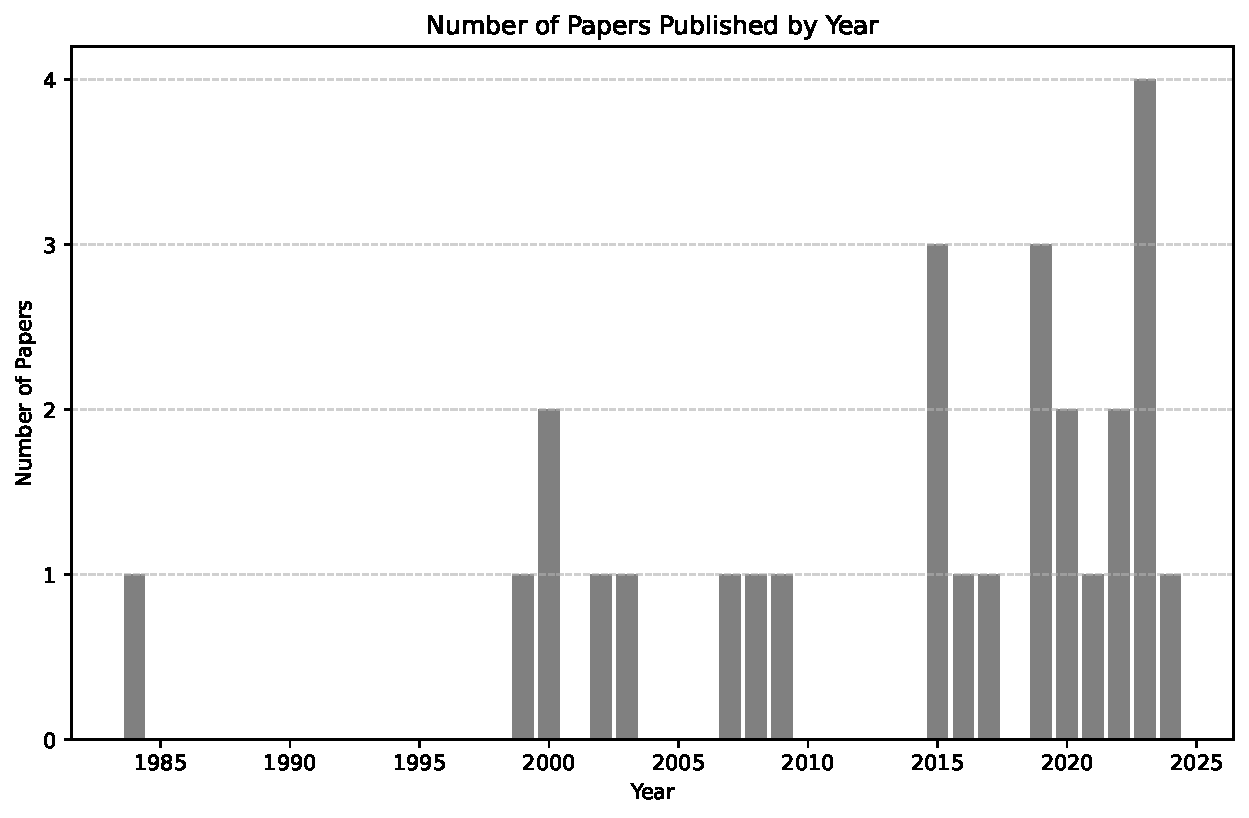
\includegraphics[width=0.99\textwidth]{figures/question_catalog/papers_by_year.pdf}
    \caption[Distribution of Papers by Publication Year]{The distribution of papers by their year of publication.}
    \label{fig:papers_by_year}
\end{figure}

\autoref{fig:papers_by_year} shows the distribution by publication year for the papers from which we extracted classes. The years range from 1984 to 2024, with most publications published in the last decade. The oldest paper is authored by \textcite{dillon_classification_1984}, who investigated the classification of research questions as suggested by Aristotle. The most recent paper is authored by \textcite{taffa_hybrid-squad_2024}, which presents the Hybrid-SQuAD dataset designed to address scholarly \gls{qa} by combining tabular and textual data. The year 2023 yielded the most publications in our set (four papers), while other years contributed between one and three papers. Several years within the range had no publications matching our criteria.



\subsection{Distribution of Citations and References}

\begin{table}[t]
    \centering
    \begin{minipage}[t]{0.43\textwidth}
        \centering
        \begin{tabular}{l c}
            \toprule
            \textbf{Paper} & \textbf{Number of Citations} \\
            \midrule
            \cite{li_learning_2002} & \cite{auer_sciqa_2023}, \cite{bolotova_non-factoid_2022}, \cite{allam_question_2016}, \cite{chernov_linguistically_2015} \\
            \cite{dubey_lc-quad_2019} & \cite{auer_sciqa_2023}, \cite{usbeck_qald-10_2023}, \cite{banerjee_dblp-quad_2023} \\
            \cite{singhal_att_1999} & \cite{auer_sciqa_2023}, \cite{chernov_linguistically_2015} \\
            \cite{mikhailian_learning_2009} & \cite{auer_sciqa_2023}, \cite{chernov_linguistically_2015} \\
            \cite{auer_sciqa_2023} & \cite{karras_divide_2023}, \cite{taffa_hybrid-squad_2024} \\
            \cite{jaradeh_question_2020} & \cite{karras_divide_2023}, \cite{taffa_hybrid-squad_2024} \\
            \cite{bordes_large-scale_2015} & \cite{auer_sciqa_2023} \\
            \cite{riloff_rule-based_2000} & \cite{auer_sciqa_2023} \\
            \cite{sjoberg_future_2007} & \cite{karras_divide_2023} \\
            \cite{moldovan_structure_2000} & \cite{chernov_linguistically_2015} \\
            \cite{banerjee_dblp-quad_2023} & \cite{taffa_hybrid-squad_2024} \\
            \bottomrule
        \end{tabular}
        \caption[Number of Citations within Paper Selection]{The number of times a paper has been cited by another paper within $\mathcal{F}$.}
        \label{table:papers_by_citations}
    \end{minipage}
    \hfill
    \begin{minipage}[t]{0.55\textwidth}
        \centering
        \begin{tabular}{l c}
            \toprule
            \textbf{Paper} & \textbf{References} \\
            \midrule
            \cite{auer_sciqa_2023} & \cite{bordes_large-scale_2015}, \cite{dubey_lc-quad_2019}, \cite{li_learning_2002}, \cite{singhal_att_1999}, \cite{riloff_rule-based_2000}, \cite{mikhailian_learning_2009} \\
            \cite{chernov_linguistically_2015} & \cite{singhal_att_1999}, \cite{moldovan_structure_2000}, \cite{mikhailian_learning_2009}\\
            \cite{karras_divide_2023} & \cite{sjoberg_future_2007}, \cite{auer_sciqa_2023}, \cite{jaradeh_question_2020} \\
            \cite{taffa_hybrid-squad_2024} & \cite{auer_sciqa_2023}, \cite{banerjee_dblp-quad_2023}, \cite{jaradeh_question_2020} \\
            \cite{bolotova_non-factoid_2022} & \cite{li_learning_2002} \\
            \cite{allam_question_2016} & \cite{li_learning_2002} \\
            \cite{banerjee_dblp-quad_2023} & \cite{dubey_lc-quad_2019} \\
            \cite{usbeck_qald-10_2023} & \cite{dubey_lc-quad_2019} \\
            \bottomrule
        \end{tabular}
        \caption[Number of References within Paper Selection]{The number of times a paper has referenced another paper within $\mathcal{F}$.}
        \label{table:papers_by_references}
    \end{minipage}
\end{table}


\autoref{table:papers_by_citations} illustrates the frequency with which the papers in our selected set ($\mathcal{F}$) cite each other. This provides insight into the relative influence of each publication within our selection. In particular, \cite{li_learning_2002} is the most frequently cited paper, indicating a potentially greater influence within our selected set of papers. In addition, five papers are cited twice and five are cited once, suggesting a modest influence within the set. Of the 27 papers in the final list, 16 were not cited by any other paper within this set, suggesting that they have had limited direct influence on the classification schemes developed in the cited works within our collection.

In contrast, \autoref{table:papers_by_references} details how often each paper references other publications within our selection. This data reveals the extent to which the classifications may have been informed by prior work. According to the data, \cite{auer_sciqa_2023} stands out with six references, indicating that its classifications are heavily influenced by other publications on our list. Similarly, \cite{chernov_linguistically_2015} references four papers, while both \cite{karras_divide_2023} and \cite{taffa_hybrid-squad_2024} cite three publications each. In addition, four papers \cite{bolotova_non-factoid_2022,allam_question_2016,banerjee_dblp-quad_2023,usbeck_qald-10_2023} include only one reference. Overall, with only eight out of 27 papers referencing other works in the data, it appears that most of the publications derive their insights independently.


\section{Clustering of Extracted Classes}
\label{sec:taxonomy_clustering}

After extracting 227 classes for question classification, we performed the \textsc{Clustering} phase of the taxonomy construction process. The goal of the clustering process is to semantically group classes with similar names or descriptions and to merge duplicate classes proposed by multiple publications, thereby providing an overview of the unique classes and reducing redundancy. The clustering process is carried out in two steps: \emph{Deduplication} and \emph{Categorization}, as described in Section~\ref{sec:tax_proc_clustering}.

\subsection{Deduplication Process}
In the first step, the names of the question classification classes and the descriptions provided by the respective authors were manually analyzed for similarities. All classes $\mathcal{C}$ that shared a similar or identical name and had semantically similar descriptions were grouped together. After performing this process, the 227 classes in $\mathcal{C}$ were consolidated into 96 merged classes $\hat{\mathcal{C}}$. Each merged class was then given a unique name and description by combining the names and descriptions of the classes within it.

\subsection{Categorization Process}
In the second step, we clustered the classes $\hat{\mathcal{C}}$ into categories. For this purpose, we analyzed the names and descriptions of the groups to identify commonalities. Classes that exhibited coherence were grouped into a category, resulting in a total of nine categories. Finally, based on the combined names and descriptions of the classes $\hat{\mathcal{C}}$ within the categories, we established a unique name and description for each of the categories. The detailed process is documented in our replication package \cite{schneider_replication_2025}. An overview of each category and its metadata is shown in \autoref{table:clustering_result}. In the following, we present the final categories with their names, descriptions, and characteristics.

\label{enum:cluster_1}
\paragraph{Category 1} We identified that the classes in this category are about the representation of knowledge in a \gls{kg}. It describes the granularity of the facts that the retriever needs to retrieve in order to arrive at the answer. The cluster distinguishes between two classes. First, questions that require the retrieval of multiple facts from the graph to be answered. Second, questions that require only one fact. As such, we named this category \emph{Graph Representation}. Five sources form this cluster \cite{banerjee_dblp-quad_2023,auer_sciqa_2023,dubey_lc-quad_2019,jaradeh_question_2020,bordes_large-scale_2015}. From the categories of these papers we can conclude that they originate from the development of \gls{kgqa} datasets, with most contributions emerging in the last five years. Moreover, the contributions span both the academic and general domains, suggesting a broad applicability of this distinction. 

\label{enum:cluster_2}
\paragraph{Category 2} This category contains the largest number of classes among all categories, encompassing a total of 33 classes derived from 25 different publication sources \cite{allam_question_2016,moldovan_structure_2000,steinmetz_what_2021,singhal_att_1999, dillon_classification_1984,riloff_rule-based_2000,taffa_hybrid-squad_2024,mikhailian_learning_2009,sjoberg_future_2007, nguyen_ripple_2017,chernov_linguistically_2015,li_learning_2002, shaw_writing_2003,bolotova_non-factoid_2022,banerjee_dblp-quad_2023,auer_sciqa_2023,dubey_lc-quad_2019,jaradeh_question_2020,tran_comparative_2022,easterbrook_selecting_2008,ratan_formulation_2019,kamper_types_2020,liu_taxonomy_2015,karras_divide_2023,thuan_construction_2019}. Each class categorizes a question based on the expected format and content of its answer. These classes span a wide range, including \emph{entities}, \emph{names}, \emph{dates}, \emph{monetary values}, and \emph{bibliometric numbers}. We find that some classes are addressed by multiple sources. The \emph{boolean} class is the most widely considered, appearing in 10 sources. This is followed by the Human/Person, Location, and Quantitative classes, each appearing in seven sources. The classes \emph{date} and \emph{description} are also commonly represented, with five sources each. Additionally, the classes \emph{undefined}, \emph{time}, \emph{organization}, and \emph{entity} are mentioned in four sources each. The remaining classes are referenced less frequently. Overall, we named this category \emph{answer type}.

\label{enum:cluster_3}
\paragraph{Category 3} This category consists of classes that define the types of operations a retriever must perform to arrive at an answer, such as \emph{negation}, \emph{contingencies}, \emph{counting}, and \emph{comparison}. With contributions from 17 different sources \cite{allam_question_2016,sjoberg_future_2007,banerjee_dblp-quad_2023,auer_sciqa_2023,nguyen_ripple_2017,easterbrook_selecting_2008,dillon_classification_1984, ratan_formulation_2019,kamper_types_2020,dubey_lc-quad_2019,usbeck_qald-10_2023,steinmetz_what_2021,tran_comparative_2022,bolotova_non-factoid_2022,jaradeh_question_2020,bordes_large-scale_2015,karras_divide_2023}, it is the second most prevalent cluster identified in our extraction. The majority of these sources stem from the \gls{kgqa} dataset literature, although the category is also addressed in works on question classification and in studies focused on scholarly research questions. It is primarily considered within open-domain and academic contexts but also receives attention in the software engineering domain. In addition, specialized fields such as requirements engineering and Covid-related research contribute to this category. We refer to this category as \emph{Question Types}.


\begin{sidewaystable}[p]
    \centering
    \resizebox{\textwidth}{!}{
    \begin{tabularx}{\textwidth}{p{4cm} p{1.5cm} p{1.5cm} X X X}     
        \toprule
        \textbf{Category Name} & \textbf{Classes} & \textbf{Sources} & \textbf{Domains} & \textbf{Years} & \textbf{Source Categories} \\
        \midrule
        Graph Representation & 2 & 5 & Scholarly, Open & 2015, 2019, 2020, 2023 & KGQA Dataset \\
        Answer Type & 33 & 25 & Scholarly, Open, Software Engineering, Language specific, Spoken NLP, Covid, Healthcare, Social Science, Requirements Engineering, Design Science & 1984, 1999, 2000, 2002, 2003, 2007, 2008, 2009, 2015, 2016, 2017, 2019, 2020, 2021, 2022, 2023, 2024 & Question Classifier, KGQA Dataset, Research Questions, Other \\
        Question Types & 18 & 17 & Scholarly, Open, Software Engineering, Language specific, Healthcare, Covid, Requirements Engineering & 1984, 2007, 2015, 2016, 2017, 2019, 2020, 2021, 2022, 2023 & Question Classifier, KGQA Dataset, Research Questions, Other \\
        WH-Patterns & 9 & 5 & Scholarly, Open, Covid, Language specific & 2000, 2017, 2022, 2023 & Question Classifier, KGQA Dataset \\
        Specialized KB Types & 2 & 3 & Scholarly, Open & 2019, 2021, 2023 & KGQA Dataset \\
        Research Focus & 8 & 2 & Scholarly, Software Engineering & 2003, 2024 & KGQA Dataset, Research Questions \\
        Answer Credibility & 5 & 5 & Requirements Engineering, Social Science, Healthcare, Open & 1984, 2020, 2022, 2023 & KGQA Dataset, Question Classifier, Research Questions \\
        Question Goal & 7 & 7 & Software Engineering, Design Science, Open & 2000, 2003, 2008, 2016, 2019, 2022 & Research Questions, Question Classifier \\
        Application Specific & 12 & 5 & Design Science, Language specific, Spoken NLP, Open & 2000, 2015, 2017, 2019, 2021 & Research Questions, Question Classifier, KGQA Dataset \\
        \bottomrule
    \end{tabularx}
    }
    \caption[Clustering of Extracted Classes]{Clustering Results for the Extracted Question Types from the Literature}
    \label{table:clustering_result}
\end{sidewaystable}

\label{enum:cluster_4}
\paragraph{Category 4} This category groups questions based on their interrogative form, distinguishing between different \enquote{Wh} word patterns such as \emph{what}, \emph{where}, \emph{which}, \emph{when}, \emph{who}, \emph{why}, \emph{whose}, and \emph{whom}. It is rooted in early question classification research and continues to be relevant in current studies. The cluster is derived from five different sources \cite{auer_sciqa_2023,riloff_rule-based_2000,tran_comparative_2022,nguyen_ripple_2017,moldovan_structure_2000} and spans both scholarly and general domains, with additional contributions from specialized areas such as Covid-related research and studies focused on the Vietnamese language. We refer to this fourth category as \emph{WH-Patterns}.

\label{enum:cluster_5}
\paragraph{Category 5} We named this category \emph{Specialized Knowledge Base Types}, as it comprises question classes tailored to specific \glspl{kb}. These include classes related to \gls{orkg}, SPARQL queries, and Wikidata qualifiers. Consequently, such classifications are only applicable when the question is executed against the corresponding \gls{kb}. The category is supported by three recent sources \cite{auer_sciqa_2023,steinmetz_what_2021,dubey_lc-quad_2019}, spanning both scholarly and general domains. Notably, it is exclusively addressed within the context of \gls{kgqa} dataset literature.

\label{enum:cluster_6}
\paragraph{Category 6} We refer to the category as \emph{Research Focus} as it centers on classifying questions according to their research-related focus. It includes classes such as Research Output, Development Methods, and Modeling Approaches and is supported by only two publications. The first is \cite{taffa_hybrid-squad_2024}, a 2024 contribution in the \gls{kgqa} dataset category, which specifically targets scholarly content. The second is \cite{shaw_writing_2003}, a 2003 study centered on research questions within the software engineering domain.

\label{enum:cluster_7}
\paragraph{Category 7} We refer to this category as \emph{Answer Credibility}, as it classifies questions based on the perceived truthfulness or reliability of the expected answer. It includes classes such as \emph{factual}, \emph{opinion}, \emph{debate}, \emph{conversational}, and \emph{predictive}. This cluster is supported by five sources \cite{karras_divide_2023,bolotova_non-factoid_2022,liu_taxonomy_2015,dillon_classification_1984,kamper_types_2020}, spanning domains such as requirements engineering, social sciences, healthcare, and the open domain. Most sources are from recent years, with the earliest dating back to 1984. The category is considered in \gls{kgqa} dataset literature, question classification studies, and research focusing on scholarly questions.

\label{enum:cluster_8}
\paragraph{Category 8} We refer to the eighth category as \emph{Question Goal}, as it captures the overarching intent or purpose behind a question. It includes classes such as \emph{exploratory}, \emph{reasoning}, \emph{problem solving}, and \emph{gap spotting}. This category is supported by seven sources \cite{easterbrook_selecting_2008,thuan_construction_2019,ratan_formulation_2019,shaw_writing_2003,bolotova_non-factoid_2022,moldovan_structure_2000,allam_question_2016}, spanning domains such as software engineering, design science, and the open domain. The publication years range from 2000 to 2022, reflecting both foundational and more recent work. The category is primarily addressed in question classification studies and literature focused on research question formulation.

\label{enum:cluster_9}
\paragraph{Category 9} We refer to this category as \emph{Application Specific}, as it encompasses classes that are tailored to particular applications or use cases. These include categories such as Research Question Utilization, Research Question Typology, and Outcome Artifact Classification. The category is supported by five sources \cite{thuan_construction_2019,nguyen_ripple_2017,chernov_linguistically_2015,moldovan_structure_2000,steinmetz_what_2021}, spanning domains such as design science, Vietnamese language studies, spoken natural language processing, and the open domain. The publication years range from 2000 to 2021. This category is addressed in question classification studies, research question-focused literature, and \gls{kgqa} dataset research.

\section{Relevance Assessment of Clusters}
\label{sec:relevance_of_clusters_analysis}

In this section, we present the \textsc{Relevance Assessment} phase of the taxonomy construction approach. For each category presented in the prior Section~\ref{sec:taxonomy_clustering}, we discuss the relevance to the taxonomy. This assessment is based on the established name and description of the category to determine if it aligns with the goal of the taxonomy. In particular, a category is seen as relevant if each of the following questions hold true:

\begin{enumerate}[label=\textbf{GQ\arabic*.}, leftmargin=2.5em]
    \item Does the category capture characteristics of questions to test the capabilities of \gls{kgqa} retrieval systems, or does it reflect aspects specific to the scholarly literature search domain?
    \item Can the category be generalized across different \gls{kgqa} systems and within the literature search domain?
    \item Can the classes within the category inform and guide the construction of diverse and meaningful evaluation datasets?
\end{enumerate}

In the following, we assess each category towards the questions.

\hyperref[enum:cluster_1]{\textbf{Category 1 – Graph Representation}} \\
This category captures structural aspects of question complexity by distinguishing between questions that require the retrieval of single versus multiple facts. This distinction directly impacts the complexity of the retrieval process and is broadly applicable across \gls{kgqa} systems. Moreover, it is particularly relevant in the scholarly domain, where complex questions are common. The cluster also offers concrete guidance for the construction of datasets that vary in granularity with respect to graph traversal. \\
\textit{Relevant:} \textbf{Yes}

\hyperref[enum:cluster_2]{\textbf{Category 2 – Answer Type}} \\
This category categorizes questions by the expected type of answer, such as dates, entities, quantities, or boolean values. These categories are helpful in describing the characteristics of questions in a literature search to construct diverse datasets. Furthermore, they are broadly applicable across domains and \gls{kgqa} systems. \\
\textit{Relevant:} \textbf{Yes}

\hyperref[enum:cluster_3]{\textbf{Category 3 – Question Types}} \\
This category focuses on logical and computational operations implied by a question, such as comparison, counting, or negation. These operations are central in retrieval and directly relate to the functional requirements of a retriever. The cluster generalizes across domains and offers valuable guidance for the inclusion of questions targeting different retrieval abilities. \\
\textit{Relevant:} \textbf{Yes}

\hyperref[enum:cluster_4]{\textbf{Category 4 – WH-Patterns}} \\
Although WH-patterns are commonly used in question classification, they primarily reflect linguistic surface forms rather than the underlying retrieval characteristics. Furthermore, the classes are not general enough to provide meaningful characteristics in the scholarly literature search setting. Its utility for guiding the construction of a diverse dataset is also limited. While it may promote diversity with regard to WH-forms, it is not helpful to capture the meaning of questions or reliably correspond to distinct retrieval challenges. \\
\textit{Relevant:} \textbf{No}

\hyperref[enum:cluster_5]{\textbf{Category 5 – Specialized Knowledge Base Types}} \\
This category encompasses classes that are specific to certain knowledge bases, such as Wikidata qualifiers or ORKG-specific constructs. Although these distinctions are meaningful within their contexts, they do not generalize across \gls{kgqa} systems or domains. Consequently, the cluster offers limited value for constructing broadly applicable evaluation datasets and is more reflective of system-specific constraints than question-inherent properties. \\
\textit{Relevant:} \textbf{No}

\hyperref[enum:cluster_6]{\textbf{Category 6 – Research-Focus}} \\
This category categorizes questions based on their orientation towards research-related topics such as research methods or modeling approaches. Although the classes may be domain-specific, they align closely with our focus on scholarly literature search. In addition, the cluster is relevant for designing evaluation datasets that capture the diversity of scholarly questions. \\
\textit{Relevant:} \textbf{Yes}

\hyperref[enum:cluster_7]{\textbf{Category 7 – Answer Credibility}} \\
This category considers the credibility of expected answers, such as factual, predictive, or opinion-based. Because the literature search can include various credibility types, this classification is relevant to the scholarly literature search and generalizable across different domains. Moreover, considering this classification promotes diversity in the creation of question datasets. \\
\textit{Relevant:} \textbf{Yes} 

\hyperref[enum:cluster_8]{\textbf{Category 8 – Question Goal}} \\
This category addresses the underlying intent behind a question, such as problem solving, reasoning, or exploration. These types of goals are relevant for scholarly literature search to capture the intent behind the question. As such, it promotes diversity in question dataset creation. \\
\textit{Relevant:} \textbf{Yes}

\hyperref[enum:cluster_9]{\textbf{Category 9 – Application-Specific}} \\
This category includes classes that are defined in relation to specific applications or use contexts, such as outcome artifact classification or research question typologies. Although these categories may be useful within individual domains, they do not reflect generalizable properties of the questions themselves. \\
\textit{Relevant:} \textbf{No}

Based on the analysis of category relevance, we conclude that six out of a total of nine identified categories can be considered relevant. Each of these categories further comprises a number of classes. For each individual class, a relevance assessment was also performed, with the detailed results documented in our replication package \cite{schneider_replication_2025}. In total, 96 classes within the categories were examined, of which 58 were rated as relevant and 38 as not relevant. This yields a class-level relevance ratio of:

\[
\text{Relevance}_\text{classes} = \frac{|\text{relevant classes}|}{|\text{total classes}|} = \frac{58}{96} \approx 0.6
\]

This indicates that approximately 60\% of the classes extracted from the literature are considered relevant for our taxonomy. A similar pattern emerges at the category level. The relevance ratio for categories is given by

\[
\text{Relevance}_\text{categories} = \frac{|\text{relevant categories}|}{|\text{total categories}|} = \frac{6}{9} = \frac{2}{3} \approx 0.66
\]

This indicates that a substantial portion of the identified categories are meaningful for structuring our taxonomy.


\section{Taxonomy Construction and Refinement}
\label{sec:taxonomy_design_construction}

This section documents the \textsc{Taxonomy Construction and Refinement} phase of the taxonomy construction approach. The first increment of the taxonomy was initialized based on the relevant categories from Section~\ref{sec:relevance_of_clusters_analysis}. We then identified several shortcomings of the taxonomy, which led to two more refinement steps until we were satisfied with the result. In the following sections, we describe each of the three increments that led to the final \gls{kgqa} retrieval taxonomy.

\subsection{First Taxonomy Increment}

The following sections will introduce the construction and validation of the first taxonomy increment.

\begin{table}[t]
\centering
\resizebox{\textwidth}{!}{%
\begin{tabular}{|l|lll|}
\hline
\textbf{Category} & \multicolumn{3}{l|}{\textbf{Classes}} \\
\hline
\begin{tabular}[c]{@{}l@{}}Graph \\ Representation\end{tabular} & \multicolumn{2}{l|}{Single Fact} & Multi Fact \\
\hline
\multirow{11}{*}{Answer Type} & \multicolumn{1}{l|}{Undefined} & \multicolumn{1}{l|}{Date} & Tool/Notation \\ \cline{2-4} 
 & \multicolumn{1}{l|}{Definition} & \multicolumn{2}{l|}{Theoretical Framework} \\ \cline{2-4} 
 & \multicolumn{1}{l|}{Abbreviation} & \multicolumn{1}{l|}{Instructional} & \multicolumn{1}{l|}{Actor} \\ \cline{2-4} 
 & \multicolumn{1}{l|}{Boolean} & \multicolumn{1}{l|}{Entity} & Human/Person \\ \cline{2-4} 
 & \multicolumn{1}{l|}{Quantitative} & \multicolumn{1}{l|}{Solution} & Time \\ \cline{2-4} 
 & \multicolumn{1}{l|}{Title} & \multicolumn{1}{l|}{Monetary} & Name \\ \cline{2-4} 
 & \multicolumn{1}{l|}{Properties} & \multicolumn{1}{l|}{Description} & Organization \\ \cline{2-4} 
 & \multicolumn{1}{l|}{Technology} & \multicolumn{1}{l|}{Software System} & Duration \\ \cline{2-4} 
 & \multicolumn{1}{l|}{Location} & \multicolumn{2}{l|}{Distance Measurement} \\ \cline{2-4} 
 & \multicolumn{1}{l|}{Other} & \multicolumn{2}{l|}{Bibliometric Numbers} \\ \cline{2-4} 
 & \multicolumn{3}{l|}{Procedure/Technique}  \\ 
 \hline
\multirow{4}{*}{Question Type} & \multicolumn{1}{l|}{Negation} & \multicolumn{1}{l|}{Dependency} & Contingency \\ \cline{2-4} 
 & \multicolumn{1}{l|}{Superlative} & \multicolumn{1}{l|}{Comparison} & Listing \\ \cline{2-4} 
 & \multicolumn{1}{l|}{Ranking} & \multicolumn{1}{l|}{Multiple Intentions} & Temporal \\ \cline{2-4} 
 & \multicolumn{1}{l|}{Relationship} & \multicolumn{1}{l|}{Counting} & Aggregation \\ 
 \hline
\multirow{2}{*}{Research Focus} & \multicolumn{1}{l|}{Development Methods} & \multicolumn{1}{l|}{Qualitative Modeling} & Analytical Methods \\ \cline{2-4} 
 & \multicolumn{1}{l|}{Generalization} & \multicolumn{1}{l|}{Analytic Modeling} & Empirical Modeling \\
 \hline
\multirow{3}{*}{Question Goal} & \multicolumn{1}{l|}{Exploratory} & \multicolumn{1}{l|}{Reasoning} & Gap Spotting \\ \cline{2-4} 
 & \multicolumn{1}{l|}{Problematization} & \multicolumn{2}{l|}{Method Improvement} \\ \cline{2-4} 
 & \multicolumn{3}{l|}{Problem Solving} \\
 \hline
\multirow{2}{*}{Answer Credibility} & \multicolumn{1}{l|}{Factual} & \multicolumn{1}{l|}{Debate} & Conversational \\ \cline{2-4} 
 & \multicolumn{1}{l|}{Predictive} & \multicolumn{2}{l|}{Opinion}  \\ 
 \hline
\end{tabular}%
}
\caption[Categories and Classes of the First Taxonomy Increment]{The categories and classes of the first taxonomy increment $\mathcal{T}_1$}
\label{tab:taxonomy_iteration_1}
\end{table}

\subsubsection{Construction of the First Taxonomy Increment}
According to the applied construction approach, the first increment of the taxonomy should be created solely using the categories classified as relevant in the \textsc{Relevance Assessment} phase. As such, the first increment of the taxonomy $\mathcal{T}_1$ is initialized with the categories that we consider relevant based on the consideration of relevance in Section~\ref{sec:relevance_of_clusters_analysis}. The first increment of the taxonomy is illustrated in \autoref{tab:taxonomy_iteration_1} and consists of six categories and 58 classes.

% \emph{Knowledge Representation}, \emph{Answer Type}, \emph{Question Type}, \emph{Research Focus}, \emph{Answer Credibility}, and \emph{Question Goal}. 

\subsubsection{Validation of the First Taxonomy Increment} 

\begin{sloppypar}
The validation is guided by the questions \hyperref[tab:gqm_taxonomy_validation]{\textbf{Q1-5}} which are presented in the \gls{gqm} plan shown in \autoref{tab:gqm_taxonomy_validation}. We indicate the taxonomy as $\mathcal{T}_1$, the classes of the taxonomy as $\mathcal{C}_{\mathcal{T}_1}$, and the objects under study as $\mathcal{C}$, which are the classes that were extracted from the literature survey. The generality (\hyperref[tab:gqm_taxonomy_validation]{\textbf{Q1.1}}) concerns whether the taxonomy is general enough, measured using \emph{laconicity} (\hyperref[tab:gqm_taxonomy_validation]{\textbf{M1.1.1}}) and \emph{lucidity} (\hyperref[tab:gqm_taxonomy_validation]{\textbf{M1.1.2}}). The laconicity measures $laconicity(\mathcal{T}_1, \mathcal{C}) = \frac{227}{227} = 1.00$, which is the maximum score that can be reached. Therefore, this indicates that no two classes from the literature appear more than once in the taxonomy, suggesting that there is no redundancy. This is to be expected given the cluster-based approach that was applied to initialize the taxonomy because each cluster was derived directly from classes extracted in the literature and no literature class is included in more than one cluster. Only the presence of such an overlap would reduce the laconicity score. Regarding the lucidity with the given $\mathcal{C}_{\mathcal{T}_1}$ and $\mathcal{C}$, we measure $lucidity(\mathcal{C}_{\mathcal{T}_1}, \mathcal{C}) = \frac{28}{58} = 0.48$. Based on this result, we can see that approximately half of the classes in the taxonomy are referenced by more than one literature source. Even though the interpretation of the metric would indicate a bad generality, we argue that in our case, this is a positive indication as it demonstrates that a significant portion of the taxonomy is supported by multiple sources. 
\end{sloppypar}

\begin{sloppypar}
The next question \hyperref[tab:gqm_taxonomy_validation]{\textbf{Q1.2}} is about the appropriateness of the taxonomy. We measure the \emph{completeness} (\hyperref[tab:gqm_taxonomy_validation]{\textbf{M1.2.1}}) score as $completeness(\mathcal{C}_{\mathcal{T}_1}, \mathcal{C}) = \frac{135}{227} = 0.59$. The score indicates that more than half of the types that we extracted from the literature have been included in some way in the taxonomy. The remaining types are not relevant to our taxonomy and, as such, are excluded from the taxonomy. For the \emph{soundness} (\hyperref[tab:gqm_taxonomy_validation]{\textbf{M1.2.2}}), we measure $soundness(\mathcal{C}_{\mathcal{T}_1}, \mathcal{C}) = \frac{58}{58} = 1.00$. The score is maximal, which is to be expected, as only in cases where a class from the taxonomy would not map to a class from the literature the soundness metric would be negatively affected and this does not happen because of the clustering approach.
\end{sloppypar}
\begin{sloppypar}
Question \hyperref[tab:gqm_taxonomy_validation]{\textbf{Q1.3}} addresses the concept of \emph{orthogonality}, which quantifies the number of overlapping classes within the taxonomy. We assess \emph{orthogonality} (\hyperref[tab:gqm_taxonomy_validation]{\textbf{M1.3.1}}) using an orthogonality matrix, calculated as $orthogonality(\mathcal{C}_{\mathcal{T}_1}, \mathcal{C}) = \frac{3176}{3306} = 0.96$, where the numerator represents orthogonal classes without overlap. Out of 3306 cases, 130 instances are identified as overlapping. We identified a total of 10 overlaps between the \emph{Question Type} category and the \emph{Multi Fact} class. These overlaps arise because certain operations, such as \emph{Dependency}, \emph{Listing}, or \emph{Aggregation}, require multiple facts from the graph. We acknowledge these overlaps but consider them acceptable, as the categories capture distinct but relevant dimensions of question classification in the context of \gls{kgqa}. Within the category \emph{Question Type} itself, additional overlaps were observed. Specifically, both \emph{Contingency} and \emph{Dependency} imply the presence of \emph{Relationship}, making this classification redundant. Therefore, a refinement for these classes is needed. There is also overlap between the classes \emph{Superlative}, \emph{Ranking}, and \emph{Counting}. All of these classes are based on the counting operation. However, they differ in terms of complexity and retrieval intent. Therefore, while they share underlying operations, each class represents a distinct capability in the retrieval process. Therefore, we argue in favor of maintaining their separation despite functional similarities.
\end{sloppypar}

\begin{table}[t]
\centering
\begin{tabular}{@{}lll@{}}
\toprule
\textbf{Question} & \textbf{Metric} & \textbf{Result}\\ 
    \midrule
    \multirow{2}{*}{\textbf{Q1.1} Generality} & \textbf{M1.1.1} Laconicity & $1.00$ \\
    & \textbf{M1.1.2} Lucidity & $0.48$ \\ 
    
    \multirow{2}{*}{\textbf{Q1.2} Appropriateness} & \textbf{M1.2.1} Completeness & $0.59$ \\
    & \textbf{M1.2.2} Soundness & $1.00$ \\ 
    
    \textbf{Q1.3} Orthogonality & \textbf{M1.3.1} Orthogonality Matrix & $0.96$\\

    \textbf{Q2.1} Relevance & \textbf{M2.1.1} Fraction of Relevance & $1.00$ \\
    
    \multirow{2}{*}{\textbf{Q2.2} Novelty} & \textbf{M2.2.1} Innovation & $0.00$\\
    & \textbf{M2.2.2} Adaption & $1.00$\\
    \bottomrule
\end{tabular}%
\caption[Validation Results of the first Taxonomy Increment]{Results of the validation for $\mathcal{T}_1$}
\label{tab:validation_t1}
\end{table}

Moreover, we identify a high degree of overlap involving the classes \emph{Entity} and \emph{Name}. These classes are intended to classify questions that inquire about a specific entity. Given that we assume that an entity always has a name, the expected answer to the question involves naming this entity, which is why the number of overlaps is high. These overlaps include 13 classes from the \emph{Answer Type} category, including \emph{Technology}, \emph{Human/Person}, \emph{Software System}, or \emph{Location}. Additionally, all classes in the \emph{Research Focus} category overlap with \emph{Entity} and \emph{Name}. These observations highlight the need to refine both categories to reduce redundancy. Overlaps are also found in the \emph{Answer Credibility} category. First, \emph{Debate} is about the provocation of discussion or argumentation rather than providing a factual answer. This naturally aligns it with the \emph{Opinion} class. Second, the \emph{Predictive} class can be based on facts or opinions, which makes the class redundant to the \emph{Factual} and \emph{Opinion} classes. In addition, predictions can represent the goal of a question rather than a type of answer credibility. For these reasons, we suggest relocating \emph{Predictive} to the \emph{Question Goal} category. In the category \emph{Question Goal}, we identify redundancies for the classes \emph{Gap Spotting} and \emph{Problematization}, as both seek to identify shortcomings or problems in the existing literature. Therefore, we see the need to combine these classes. Furthermore, we identify 36 overlaps with the \emph{Exploratory} class, which can be attributed to its broad definition. Given the nature of many \gls{kgqa} questions, one could argue that their primary purpose is to explore the \gls{kg} in order to retrieve answers. We therefore argue that the \emph{Exploratory} class should be removed due to its overly general nature.

\begin{sloppypar}
The next question \hyperref[tab:gqm_taxonomy_validation]{\textbf{Q1.4}} is about the \emph{relevance} (\hyperref[tab:gqm_taxonomy_validation]{\textbf{M2.1.1}}) of the taxonomy. Because we initialized the taxonomy based on a relevance analysis, we argue that all classes in the taxonomy are relevant to our cause. Therefore, we measure $relevance(\mathcal{C}_{\mathcal{T}_1}, \mathcal{C}) = \frac{58}{58} = 1.00$, which is the maximal score.
\end{sloppypar}

\begin{sloppypar}
Whether the taxonomy reached an appropriate novelty (\hyperref[tab:gqm_taxonomy_validation]{\textbf{Q1.5}}) is measured with the innovation and adaptation metrics. Concerning \emph{innovation} (\hyperref[tab:gqm_taxonomy_validation]{\textbf{M2.2.1}}), we measure $innovation(\mathcal{C}_{\mathcal{T}_1}, \mathcal{C}) = \frac{0}{58} = 0.00$, the lowest possible value. With regard to \emph{adaption} (\hyperref[tab:gqm_taxonomy_validation]{\textbf{M2.2.2}}), we measure $adaptation(\mathcal{C}_{\mathcal{T}_1}, \mathcal{C}) = \frac{58}{58} = 1.00$, the highest possible value. This means that the taxonomy does not provide innovation and is fully adapted from the literature. This is an expected outcome, as the first increment of the taxonomy consists only of categories and classes from the literature.
\end{sloppypar}


\subsection{Second Taxonomy Increment}

When validating the first taxonomy increment $\mathcal{T}_1$, we found that there are issues with orthogonality. Some of the classes have overlaps, leading to redundancies and difficulties in the application. To solve these problems, we create the second increment $\mathcal{T}_2$ of the taxonomy, which is shown in \autoref{tab:taxonomy_t2}. In the following, we discuss the changes and validate the result.

\begin{table}[t]
\centering
% \resizebox{\textwidth}{!}{%
\begin{tabular}{|l|lll|}
\hline
\textbf{Category} & \multicolumn{3}{l|}{\textbf{Classes}} \\ \hline

\begin{tabular}[c]{@{}l@{}}Graph \\ Representation\end{tabular} & \multicolumn{2}{l|}{Single Fact} & Multi Fact \\ \hline

\multirow{2}{*}{Answer Type} & \multicolumn{1}{l|}{Named Entity} & \multicolumn{1}{l|}{Description} & Temporal \\ \cline{2-4} 
 & \multicolumn{1}{l|}{Quantitative} & \multicolumn{1}{l|}{Boolean} & Other Type \\ \cline{2-4} 
 \hline
 
\multirow{2}{*}{Answer Format} & \multicolumn{1}{l|}{Simple} & \multicolumn{1}{l|}{Enumerative} & Other Format \\ \cline{2-4} 
& \multicolumn{3}{l|}{Explanatory} \\ \hline
 
\multirow{3}{*}{Question Type} & \multicolumn{1}{l|}{Negation} & \multicolumn{1}{l|}{Counting} & Aggregation  \\ \cline{2-4} 
 & \multicolumn{1}{l|}{Superlative} & \multicolumn{1}{l|}{Comparison} & Relationship \\ \cline{2-4} 
 & \multicolumn{1}{l|}{Multiple Intentions} & \multicolumn{1}{l|}{Ranking} & Temporal \\
 
% \multirow{3}{*}{Research Focus} & \multicolumn{2}{l|}{Methodological Approaches} & Other \\ \cline{2-4} 
%  & \multicolumn{3}{l|}{Modeling Approaches} \\ \cline{2-4} 
%  & \multicolumn{3}{l|}{Conceptual Foundations} \\ 
\hline
 
\multirow{2}{*}{Question Goal} & \multicolumn{1}{l|}{Problem Solving} & \multicolumn{1}{l|}{Reasoning} & Improvement \\ \cline{2-4} 
 & \multicolumn{1}{l|}{Prediction} & \multicolumn{2}{l|}{Problematization} \\ 
 \hline
 
Answer Credibility & \multicolumn{1}{l|}{Subjective} & \multicolumn{2}{l|}{Objective}  \\ 
 \hline
\end{tabular}%
% }
\caption[Categories and Classes of the Second Taxonomy Increment]{The categories and classes of the second taxonomy increment $\mathcal{T}_2$}
\label{tab:taxonomy_t2}
\end{table}

\subsubsection{Construction of the Second Taxonomy Increment}
The construction of the second taxonomy increment $\mathcal{T}_2$ is based on a refinement of the issues identified in the first increment $\mathcal{T}_1$. In the following, we discuss the changes that were applied.

\paragraph{Consolidation of Entity-Related Classes}

In the first increment of the taxonomy ($\mathcal{T}_1$), it became evident that the classes \emph{Entity} and \emph{Name} exhibit a significant overlap within the taxonomy. This can be attributed to the fact that both classes are defined in a highly generic manner, and many more specific classes ultimately involve identifying the name of an entity. For example, questions concerning a software tool, an organization, or a scientific paper can all be interpreted as inquiries about nameable entities.

To address this in the second increment ($\mathcal{T}_2$), we consolidated these overlapping classes under a new, higher-level class: \emph{Named Entity}. This decision was guided by the goal of the \emph{Answer Type} category, which is to classify questions based on the type of information expected in the answer. Questions such as \enquote{Which software is used for X?} or \enquote{What is the title of the paper from Y?} illustrate different entities but share the commonality of seeking a name. Furthermore, highly granular classes like \emph{Software Tool}, \emph{Organization}, or \emph{Paper} reduce the generalizability of the taxonomy, as this abstraction level makes it difficult to reach a state of completeness. Moreover, such fine distinctions do not meaningfully impact the retrieval process, as the central objective remains the identification of the name of an entity. Consequently, we argue that the specific semantic content of the name is irrelevant to the underlying retrieval mechanics.

The consolidation into the \emph{Named Entity} class encompasses a total of 18 classes. This includes all classes from the \emph{Research Focus} category and 11 classes from \emph{Answer Type}. We also merged the \emph{Date}, \emph{Time}, and \emph{Duration} classes into a single class \emph{Temporal}, as all of them classify by a specific point or range in time. Moreover, we merged all quantification classes into the \emph{Quantitative} class to reduce redundancy and keep the same level of abstraction across the category. Lastly, we consolidated the classes \emph{Theoretical Framework}, \emph{Tool/Notation}, \emph{Description}, and \emph{Definition} into a single class named \emph{Description}. This new type should capture those answers that are descriptive in nature, meaning that their goal is to describe or explain something using one or more comprehensive natural language sentences. 

The classes in the \emph{Answer Type} category are now \emph{Named Entity}, \emph{Description}, \emph{Temporal}, \emph{Quantitative}, \emph{Boolean}, and \emph{Other Type}. We consider these classes to be orthogonal to each other and argue that each represents different complexities in the \gls{kgqa} retrieval process. This allows for the classification of questions according to whether they seek a name, a description, a date or time span, quantitative data, Boolean data, or another type of information..

\paragraph{Introduction of the Answer Format Category}
The second increment of the taxonomy ($\mathcal{T}_2$) introduces a new category, which we refer to as \emph{Answer Format}. This category classifies questions according to their expected format or structure of the answer. It emerged from the observation that three classes in $\mathcal{T}_1$ described the format of the answer rather than its content, making their original categorization semantically inconsistent. This applies to the class \emph{Instructional}, which classifies whether an answer is expected to be a step-by-step sequence of instructions. Furthermore, it concerns the classes \emph{Properties} and \emph{Listing}, both of which expect an answer in the form of an enumeration. These three are therefore combined into a new class called \emph{Enumerative}.

To increase the completeness of the new category, we introduce three additional classes: \emph{Simple}, \emph{Explanatory}, and \emph{Other Format}. The class \emph{Simple} classifies questions that expect a direct, brief, and minimalistic answer. These are typically answers consisting of a single sentence that conveys a factual statement without further explanation. The class \emph{Explanatory} classifies questions for which the expected answer is a textual explanation of a phenomenon or an entity. Finally, we introduce the new class \emph{Other Format} to cover all answer formats that have not been considered in the category thus far.

\paragraph{Refinement of Answer Credibility}
In the second increment $\mathcal{T}_2$, we refine the \emph{Answer Credibility} dimension by reducing it to the classes \emph{Subjective} and \emph{Objective}. The classes \emph{Debate} and \emph{Opinion} were merged into \emph{Subjective}, while \emph{Factual} was renamed to \emph{Objective} to clearly contrast with subjective responses. This change aims to improve clarity by emphasizing the binary nature of the perceived credibility of the answer.

\paragraph{Adjustments to Question Goal}
During the validation of the first taxonomy increment ($\mathcal{T}_1$), the \emph{Exploratory} class was found to be overly broad, leading to significant overlaps with other classes. As most research questions are exploratory to some degree, we argue that the class lacks discriminative power, which is why we removed it.

Furthermore, the classes \emph{Problematization} and \emph{Gap Spotting} were merged, as both aim to identify shortcomings or gaps in existing literature. Moreover, to resolve inconsistencies in the abstraction levels in the category, we renamed \emph{Method Improvement} to \emph{Improvement}, aligning it with the general abstraction level used in the category.

Lastly, the \emph{Prediction} class, originally part of \emph{Answer Credibility}, was moved to \emph{Question Goal}. This shift reflects its stronger alignment with the intent of the question rather than the credibility of the answer and helps to complete the conceptual space covered by \emph{Question Goal}.

\subsubsection{Validation of the Second Taxonomy Increment}

\begin{table}[t]
\centering
\begin{tabular}{@{}lll@{}}
\toprule
\textbf{Question} & \textbf{Metric} & \textbf{Result}\\ 
    \midrule
    \multirow{2}{*}{\textbf{Q1.1} Generality} & \textbf{M1.1.1} Laconicity & $1.00$ \\
    & \textbf{M1.1.2} Lucidity & $0.25$ \\ 
    
    \multirow{2}{*}{\textbf{Q1.2} Appropriateness} & \textbf{M1.2.1} Completeness & $0.57$ \\
    & \textbf{M1.2.2} Soundness & $0.89$ \\ 
    
    \textbf{Q1.3} Orthogonality & \textbf{M1.3.1} Orthogonality Matrix & $0.98$\\

    \textbf{Q2.1} Relevance & \textbf{M2.1.1} Fraction of Relevance & $1.00$ \\
    
    \multirow{2}{*}{\textbf{Q2.2} Novelty} & \textbf{M2.2.1} Innovation & $0.11$\\
    & \textbf{M2.2.2} Adaption & $0.89$\\
    \bottomrule
\end{tabular}%
\caption[Validation Results of the Second Taxonomy Increment]{Results of the validation for $\mathcal{T}_2$}
\label{tab:validation_t2}
\end{table}

\begin{sloppypar}
    Guided by the questions \hyperref[tab:gqm_taxonomy_validation]{\textbf{Q1-5}} from the \gls{gqm} plan shown in \autoref{tab:gqm_taxonomy_validation}, we are discussing the validation of the second increment of the taxonomy ($\mathcal{T}_2$). Regarding the \emph{lucidity} (\hyperref[tab:gqm_taxonomy_validation]{\textbf{M1.1.2}}), the new increment measures $lucidity(\mathcal{C}_{\mathcal{T}_2}, \mathcal{C}) = \frac{7}{28} = 0.25$, which is $0.23$ less than in the first increment. This drop in score is the result of the merges of classes, as 21 out of 28 classes in the taxonomy can be mapped to more than one class from the literature. Still, we consider these merges to be justified because we were able to reduce a large number of redundancies, making the taxonomy more interpretable and usable. Moreover, as we argued before, we consider a low \emph{lucidity} to be good in our case, as this indicates that a high number of classes in our taxonomy are supported by multiple sources in the literature. The \emph{laconicity} (\hyperref[tab:gqm_taxonomy_validation]{\textbf{M1.1.1}}), on the other hand, stays the same as in the first increment $\mathcal{T}_1$. 

    We argue that regarding the \emph{generality} (\hyperref[tab:gqm_taxonomy_validation]{\textbf{Q1.1}}) of the taxonomy, we reached an appropriate level. By applying the merges to the classes, we were also able to reduce the number of classes from 58 to 28 classes, an overall reduction of approximately $52\%$. We assert that the remaining classes provide a high level of generality, making it less likely that classes are present that are never used during application.
\end{sloppypar}

\begin{sloppypar}
    With regard to the \emph{appropriateness} (\hyperref[tab:gqm_taxonomy_validation]{\textbf{Q1.2}}), we measure \emph{completeness} (\hyperref[tab:gqm_taxonomy_validation]{\textbf{M1.2.1}}) $completeness(\mathcal{C}_{\mathcal{T}_2}, \mathcal{C}) = \frac{130}{227} = 0.57$. This is a reduction of $0.02$ compared to the first increment $\mathcal{T}_1$, which is the result of the removal of the \emph{Exploratory} class, as this class corresponds to five classes from the literature. However, we see this removal as justified, as it reduces the overall amount of dependencies, which improves the orthogonality of the taxonomy. 

    Furthermore, for the \emph{soundness} (\hyperref[tab:gqm_taxonomy_validation]{\textbf{M1.2.2}}) we measure $soundness(\mathcal{C}_{\mathcal{T}_2}, \mathcal{C}) = \frac{25}{28} = 0.89$, which is a reduction of $0.11$ in comparison to the first increment $\mathcal{T}_1$. This is the result of introducing three new classes: \emph{Simple}, \emph{Explanatory} and \emph{Other Format} to the taxonomy, which are not covered by the literature. We argue that the additions improve the overall generality of the taxonomy, making it more reliably applicable. 
\end{sloppypar}

\begin{sloppypar}
    We measure \emph{orthogonality} (\hyperref[tab:gqm_taxonomy_validation]{\textbf{M1.3.1}}) using the orthogonality matrix as $orthogonality(\mathcal{C}_{\mathcal{T}_2}, \mathcal{C}) = \frac{745}{756} = 0.98$. We observe that 11 classes have overlaps, which is a significant reduction from the previous 130 overlaps identified in the first increment $\mathcal{T}_1$. The remaining overlaps concern classes from the \emph{Question Type} category with the \emph{Multi Fact} class and within the \emph{Question Type} category itself. As we argued before, we think that this overlap is justified because of the differences in complexity that they impose on the retrieval.
\end{sloppypar}

\begin{sloppypar}
    Regarding \emph{relevance} (\hyperref[tab:gqm_taxonomy_validation]{\textbf{M2.1.1}}), we argue that the relevance of previous classes remains the same. Furthermore, we identify the three new classes that have been added in this increment as relevant for \gls{kgqa} retrieval, as they assess the ability of the retriever to present the answers in different ways. Therefore, we measure the $relevance(\mathcal{C}_{\mathcal{T}_2}, \mathcal{C}) = \frac{28}{28} = 1.00$.
\end{sloppypar}

\begin{sloppypar}
    The addition of three new classes increased the \emph{innovation} (\hyperref[tab:gqm_taxonomy_validation]{\textbf{M2.2.1}}) of the taxonomy which we measure as $innovation(\mathcal{C}_{\mathcal{T}_2}, \mathcal{C}) = \frac{3}{28} = 0.11$. Consequently, it reduced \emph{adaptation} (\hyperref[tab:gqm_taxonomy_validation]{\textbf{M2.2.2}}) by $0.11$, which we measure as $adaptation(\mathcal{C}_{\mathcal{T}_2}, \mathcal{C}) = \frac{25}{28} = 0.89$.
\end{sloppypar}

In summary, scores with respect to \emph{generality}, \emph{appropriateness} and \emph{orthogonality} reached a satisfactory point. However, regarding the novelty of the taxonomy, we observe that there is a need to add some missing classes to improve the applicability of the taxonomy. Furthermore, we identify that the \emph{Question Type} dimension contains multiple intentions and may be subject to a name change. As such, we conduct a third increment to improve these areas of the taxonomy.

\subsection{Third Taxonomy Increment}

In the third increment of the taxonomy, two new categories are introduced: \emph{Condition Constraint} and \emph{Intention Count}. In addition, four new classes are added: \emph{Basic}, \emph{Other Goal}, \emph{Information Lookup} \emph{Normative} and \emph{Single Intention}. Furthermore, the \emph{Question Type} category has been renamed to \emph{Retrieval Operation}. We discuss these changes in the following.

\begin{table}[t]
\centering
% \resizebox{\textwidth}{!}{%
\begin{tabular}{|l|lll|}
\hline
\textbf{Category} & \multicolumn{3}{l|}{\textbf{Classes}} \\ \hline

\begin{tabular}[c]{@{}l@{}}Graph \\ Representation\end{tabular} & \multicolumn{2}{l|}{Single Fact} & Multi Fact \\ \hline

\multirow{2}{*}{Answer Type} & \multicolumn{1}{l|}{Named Entity} & \multicolumn{1}{l|}{Description} & Temporal\\ \cline{2-4} 
 & \multicolumn{1}{l|}{Quantitative} & \multicolumn{1}{l|}{Boolean} & Other Type  \\ \cline{2-4} 
 \hline

 \multirow{2}{*}{Condition Type} & \multicolumn{1}{l|}{Named Entity} & \multicolumn{1}{l|}{Description} & Temporal\\ \cline{2-4} 
 & \multicolumn{1}{l|}{Quantitative} & \multicolumn{2}{l|}{Other Type} \\ \cline{2-4} 
 \hline
 
\multirow{2}{*}{Answer Format} & \multicolumn{1}{l|}{Simple} & \multicolumn{1}{l|}{Enumerative} & Other Format \\ \cline{2-4} 
& \multicolumn{3}{l|}{Explanatory} \\ \hline
 
\multirow{3}{*}{Retrieval Operation} & \multicolumn{1}{l|}{Basic} & \multicolumn{1}{l|}{Counting} & Aggregation  \\ \cline{2-4} 
 & \multicolumn{1}{l|}{Superlative} & \multicolumn{1}{l|}{Comparison} & Relationship \\ \cline{2-4} 
 & \multicolumn{1}{l|}{Negation} & \multicolumn{2}{l|}{Ranking} \\
\hline

\multirow{1}{*}{Intention Count} & \multicolumn{1}{l|}{Single Intention} & \multicolumn{2}{l|}{Multiple Intentions} \\ 
 \hline
 
\multirow{3}{*}{Question Goal} & \multicolumn{1}{l|}{Problem Solving} & \multicolumn{1}{l|}{Reasoning} & Improvement \\ \cline{2-4} 
 & \multicolumn{1}{l|}{Prediction} & \multicolumn{1}{l|}{Problematization} & \multicolumn{1}{l|}{Information Lookup} \\ \cline{2-4} 
 & \multicolumn{3}{l|}{Other Goal} \\
 \hline
 
Answer Credibility & \multicolumn{1}{l|}{Subjective} & \multicolumn{1}{l|}{Objective} & \multicolumn{1}{l|}{Normative}  \\ 
 \hline
\end{tabular}%
% }
\caption[Categories and Classes of the Third Taxonomy Increment]{The categories and classes of the third taxonomy increment $\mathcal{T}_3$}
\label{tab:taxonomy_t3}
\end{table}

\subsubsection{Construction of the Third Taxonomy Increment}

The construction of the third taxonomy increment $\mathcal{T}_3$ is based on a refinement of the issues identified in the second increment $\mathcal{T}_2$. In the following, we discuss the changes that were applied.

\paragraph{Introduction of the Condition Type Category}
We have identified a gap in the existing classification scheme: currently there is no category that captures the types of conditions that an answer must satisfy. These constraints are important because they can significantly affect the complexity of answering a question. In particular, they offer insight into how well a \gls{kgqa} approach handles multiple or diverse types of conditions.

To address this, we introduce a new dimension called \emph{Condition Type}, which classifies questions based on the types of conditions or constraints that the expected answer must meet. We hypothesize that these condition types mirror those found in the \emph{Answer Type} dimension, since both describe similar categories of information. However, we make an exception for the \emph{Boolean} class, as we argue that a condition by nature is Boolean, so this class does not fit into the new category. Therefore, we initialize the new category \emph{Condition Type} with the same set of classes as \emph{Answer Type} except for \emph{Boolean}.

\paragraph{Renaming of the Question Type Category}
We observed that the previous \emph{Question Type} category consists mostly of operations. We have therefore decided to rename the category to \emph{Retrieval Operation}. With this renaming, we want to make it clear to the reader directly from the name what this category is trying to achieve. We believe that the previous name was too abstract to achieve this goal. Furthermore, we argue that the \emph{Temporal} class in the category is not an operation but a constraint. We have therefore merged the class into the \emph{Temporal} class of the condition type category.

\paragraph{Introduction of the Intention Count Category}
We determined that the \emph{Multiple Intentions} class does not perform an operational function. Rather, it reflects the structural complexity of a question. Since it no longer aligns with the \emph{Retrieval Operation} category, we introduce the \emph{Intention Count} category. This new category classifies questions according to the number of distinct intentions they express. If a question contains a single, unified query that cannot be decomposed into separate independent questions without altering its context, it is classified as \emph{Single Intention}. In contrast, if a question can be split into two or more independent queries, it falls under \emph{Multiple Intentions}.

\paragraph{Adding Missing Classes}
We identified four missing classes in our taxonomy and introduced them in this increment. First, \emph{Basic} was added to the \emph{Retrieval Operation} category to capture questions in which the retriever should simply extract one or more factual items from the graph, without requiring further processing. Second, we introduced \emph{Normative} into the category \emph{Answer Credibility} to classify questions based on ethical, normative, or political values. Third, we added \emph{Information Lookup} to classify questions whose objective is simply to retrieve specific data from the \gls{kg} into the \emph{Question Goal} category. Finally, \emph{Other Goal} was included to accommodate questions that do not fit any other defined goal class, ensuring that all questions can be properly classified.

\subsubsection{Validation of the Third Taxonomy Increment}

\begin{table}[t]
\centering
\begin{tabular}{@{}lll@{}}
\toprule
\textbf{Question} & \textbf{Metric} & \textbf{Result}\\ 
    \midrule
    \multirow{2}{*}{\textbf{Q1.1} Generality} & \textbf{M1.1.1} Laconicity & $0.70$ \\
    & \textbf{M1.1.2} Lucidity & $0.32$ \\ 
    
    \multirow{2}{*}{\textbf{Q1.2} Appropriateness} & \textbf{M1.2.1} Completeness & $0.57$ \\
    & \textbf{M1.2.2} Soundness & $0.78$ \\ 
    
    \textbf{Q1.3} Orthogonality & \textbf{M1.3.1} Orthogonality Matrix & $0.99$\\

    \textbf{Q2.1} Relevance & \textbf{M2.1.1} Fraction of Relevance & $1.00$ \\
    
    \multirow{2}{*}{\textbf{Q2.2} Novelty} & \textbf{M2.2.1} Innovation & $0.22$\\
    & \textbf{M2.2.2} Adaption & $0.78$\\
    \bottomrule
\end{tabular}%
\caption[Validation Results of the Third Taxonomy Increment]{Results of the validation for $\mathcal{T}_3$}
\label{tab:validation_t3}
\end{table}

\begin{sloppypar}
    With regard to \emph{laconicity} (\hyperref[tab:gqm_taxonomy_validation]{\textbf{M1.1.1}}), we measure the following $laconicity(\mathcal{C}_{\mathcal{T}_3}, \mathcal{C}) = \frac{160}{227} = 0.70$, which represents a decrease of $0.30$ compared to $\mathcal{T}_2$. The reason for this reduction lies in the fact that, for the new category \emph{Condition Type}, we use the same classes as in the category \emph{Answer Type}. As a result, the metric detects a high degree of redundancy between our taxonomy and the classes from the literature. However, we consider the separation of these two categories to be justified since they address different aspects that are both essential for representing the complexity of a \gls{kgqa} retrieval.
    
    For \emph{lucidity} (\hyperref[tab:gqm_taxonomy_validation]{\textbf{M1.1.2}}), we measure $lucidity(\mathcal{C}_{\mathcal{T}_3}, \mathcal{C}) = \frac{12}{37} = 0.32$. This corresponds to an increase of $0.07$ compared to the second increment $\mathcal{T}_2$. The improvement is due to the addition of new classes that are not found in the literature, which positively influences the score. In general, we argue that the low \emph{lucidity} value is actually a positive indication for the taxonomy. This is because a high overlap with the literature indicates that our taxonomy aligns well with existing research.
    
    In general, we argue that the \emph{generality} (\hyperref[tab:gqm_taxonomy_validation]{\textbf{Q.1.1}}) has reached an appropriate level. By consolidating the classes, we achieved a consistent level of abstraction within the categories. This enables the taxonomy to be applied in a general way while maintaining enough precision to support the classification of both the capabilities of a \gls{kgqa} retrieval system and the characteristics relevant for scholarly literature search. 
\end{sloppypar}

\begin{sloppypar}
    The \emph{completeness} (\hyperref[tab:gqm_taxonomy_validation]{\textbf{M1.2.1}}) is measured as $completeness(\mathcal{C}_{\mathcal{T}_3}, \mathcal{C}) = \frac{130}{227} = 0.57$ and remains unchanged compared to the previous increment $\mathcal{T}_2$. In contrast, \emph{soundness} (\hyperref[tab:gqm_taxonomy_validation]{\textbf{M1.2.2}}) shows a value of $soundness(\mathcal{C}_{\mathcal{T}_3}, \mathcal{C}) = \frac{29}{37} = 0.78$, which represents a decrease of $0.11$ compared to the previous increment. This change can be attributed to the addition of new classes, as these are not mapped to classes from the literature.

    In general, we argue that the \emph{appropriateness} (\hyperref[tab:gqm_taxonomy_validation]{\textbf{Q1.2}}) has reached a satisfactory level. From the set of classes found in the literature, we have filtered out those that are relevant to our taxonomy. A higher level of \emph{completeness} could be achieved by including more classes from the literature in the taxonomy. However, this would negatively affect other metrics since those additional classes are not relevant to our cause. Furthermore, \emph{soundness} correlates with the \emph{novelty} of the taxonomy. This means that removing new classes from the taxonomy would increase the value but at the cost of reducing the applicability and usefulness of the taxonomy.
\end{sloppypar}

\begin{sloppypar}
    The amount of overlaps (\hyperref[tab:gqm_taxonomy_validation]{\textbf{Q1.3}}) in the taxonomy is measured with the \emph{orthogonality} (\hyperref[tab:gqm_taxonomy_validation]{\textbf{M1.3.1}}), which we measure as $orthogonality(\mathcal{C}_{\mathcal{T}_3}, \mathcal{C}) = \frac{1321}{1332} = 0.99$, amounting to 11 overlaps across the taxonomy. These overlaps are the same as in $\mathcal{T}_2$, where we already argued their appropriateness.
\end{sloppypar}

\begin{sloppypar}
    As with previous increments, the \emph{relevance} (\hyperref[tab:gqm_taxonomy_validation]{\textbf{M2.1.1}}) measures $relevance(\mathcal{C}_{\mathcal{T}_3}, \mathcal{C}) = \frac{37}{37} = 1.00$. This is because the previous classes in the taxonomy were already determined to be relevant and the new additions were included because they were missing and are relevant to our objectives.
\end{sloppypar}

\begin{sloppypar}
    Regarding the \emph{novelty} (\hyperref[tab:gqm_taxonomy_validation]{\textbf{Q2.2}}) of the taxonomy. The \emph{innovation} (\hyperref[tab:gqm_taxonomy_validation]{\textbf{M2.2.1}}) measures $innovation(\mathcal{C}_{\mathcal{T}_3}, \mathcal{C}) = \frac{8}{37} = 0.22$, indicating that 8 of the 37 classes are new, not yet considered in the classes from our literature survey. Furthermore, the \emph{adaptation} (\hyperref[tab:gqm_taxonomy_validation]{\textbf{M2.2.2}}) measures $adaptation(\mathcal{C}_{\mathcal{T}_3}, \mathcal{C}) = \frac{29}{37} = 0.78$, which states that 29 of the 37 classes were adapted from the literature.

    Overall, we are satisfied with the \emph{novelty} of the third increment $\mathcal{T}_3$ of the taxonomy. We could try to find more new classes to reach a higher \emph{innovation} score, but this would also introduce the risk of lowering the orthogonality and generality of the taxonomy.
\end{sloppypar}

\section{Categories and Classes of the Taxonomy}
\label{sec:taxonomy_final}

% Answer Type: What kind of thing the answer is.
% Constraint: What filters or conditions are applied
% Boolean: Which papers applied [Boolean] the evaluation method [Named Entity] with the name Interview?

In Section~\ref{sec:taxonomy_design_construction}, three different increments of the taxonomy were created in an iterative process. With the last increment being $\mathcal{T}_3$, which is presented in \autoref{tab:taxonomy_t3}, we have reached a satisfactory point by validating the generality (\hyperref[tab:gqm_taxonomy_validation]{\textbf{Q1.1}}), appropriateness (\hyperref[tab:gqm_taxonomy_validation]{\textbf{Q1.2}}), orthogonality (\hyperref[tab:gqm_taxonomy_validation]{\textbf{Q1.3}}), relevance (\hyperref[tab:gqm_taxonomy_validation]{\textbf{Q2.1}}), and novelty (\hyperref[tab:gqm_taxonomy_validation]{\textbf{Q2.2}}). We therefore introduce the categories and classes of the final \gls{kgqa} retrieval taxonomy in this section, before demonstrating its application in the following Section~\ref{sec:taxonomy_application}.

\subsection{Graph Representation}

\begin{table}[t]
    \centering
    \begin{tabular}{@{}lp{8cm}@{}}
        \toprule
        \textbf{Class} & \textbf{Description} \\
        \midrule
        \textbf{Single Fact}
            & Whether the answer can be found in a single fact of the \gls{kg}.\\
        \cmidrule(l){1-2}
            \textbf{Multi Fact}
            & Whether the answer must be aggregated from multiple facts in the \gls{kg}.\\
        \bottomrule
    \end{tabular}
    \caption[Graph Representation Category of the Taxonomy]{Graph representation category of the \gls{kgqa} retrieval taxonomy. It classifies questions by the amount of facts that need to be retrieved to provide a complete answer.}
    \label{tab:graph_representation}
\end{table}

The goal of the \textbf{Graph Representation} category is to classify the number of facts required to answer a given question. Here, a fact in a graph is formed by two entities connected through a relationship \cite{abu-salih_domain-specific_2021}. Specifically, in a \gls{rdf} graph, such a fact is represented as a triple consisting of $(subject, predicate, object)$ \cite{wood_rdf_2014}.

The category comprises two distinct classes, as shown in \autoref{tab:graph_representation}. The \emph{Single Fact} class is assigned when only one fact is needed, whereas the \emph{Multi Fact} class is used if multiple facts must be combined to construct the answer. These two classes are mutually exclusive, meaning that a question can be assigned to one of them only. Furthermore, it is important to note that in order to apply this category appropriately, it is essential to have knowledge of the underlying structure of the \gls{kg}. Specifically, it must be determined whether the answer to the question is represented by a single triple or spans across multiple triples within the graph.


\subsection{Answer Type}

\begin{table}[t]
    \centering
    \begin{tabular}{@{}lp{8cm}@{}}
        \toprule
        \textbf{Class} & \textbf{Description} \\
        \midrule
        \textbf{Named Entity}
            & The expected answer contains a specific named entity, such as people, organizations, locations, systems, technologies, and other concrete subjects or objects that are usually capitalized. \\
        \cmidrule(l){1-2}
            \textbf{Description}
            & The expected answer contains a descriptive phrase or sentence, such as explanations, definitions, theoretical constructs, or conceptual overviews. \\
        \cmidrule(l){1-2}
            \textbf{Temporal}
            & The expected answer refers to a specific point in time or a time range, such as dates, timestamps, or general time expressions. \\
        \cmidrule(l){1-2}
            \textbf{Quantitative}
            & The expected answer contains a numerical value, such as a measurements, monetary values, or general counts. \\
        \cmidrule(l){1-2}
            \textbf{Boolean}
            & The expected answer is binary, typically \enquote{yes} or \enquote{no}. \\
        \cmidrule(l){1-2}
            \textbf{Other Type}
            & The expected answer is of a type that does not fit into any of the other defined classes. \\
        \bottomrule
    \end{tabular}
    \caption[Answer Type Category of the Taxonomy]{Answer type category of the \gls{kgqa} retrieval taxonomy. It classifies questions by the types that are contained within the expected answer.}
    \label{tab:answer_type}
\end{table}

The \textbf{Answer Type} category serves to systematically classify questions based on the types expected in their answers. Consequently, applying this category necessitates the formulation of hypothetical answers, since the classification is determined by the inherent types present in the anticipated response. Furthermore, multiple classifications are allowed and may even be necessary for complex questions. A total of six distinct classes are defined, as presented in Table \ref{tab:answer_type}.

\emph{Named Entity} is applied when the answer contains specific named entities. This includes persons, organizations, geographical locations, as well as formal identifiers such as publication titles or Digital Object Identifiers (DOIs). An example of such a question is \enquote{What is the long form of MVC?}, which in the context of software engineering stands for \enquote{Model-View-Controller}. Since this is the name of a popular software architectural style, we can classify that the expected answer to this question is a named entity.

\emph{Description} classifies expected answers that consist of explanatory or definitional natural language expressions. These answers are formulated in complete sentences and provide detailed information about concepts, processes, or relationships. An example of this classification is the question \enquote{What does the MVC architecture pattern do?}. Because this question expects the answer to be a complete sentence explanation in natural language, it qualifies for this class.

\emph{Temporal} refers to expected answers that involve temporal expressions, either as specific points in time or as intervals of time. For example, the question \enquote{When was the MVC software architecture pattern first mentioned?} asks for a specific publication date. Because the answer is expected to provide temporal information, the class qualifies.

\emph{Quantitative} includes expected answers that contain numerical information. This can include absolute numbers, units of measurement, statistical values, or comparative quantities. An example of a question that qualifies for this class is \enquote{How much does the application of the MVC software architectural style affect the response time of the system?}. The answer to this question is expected to be a number that quantifies the change in response time. Since this is a quantitative type, the class qualifies.

\emph{Boolean} denotes expected answers that represent a binary decision. Typically, these are statements that can be answered with \enquote{yes} or \enquote{no}. This class is particularly useful for decision-making questions such as \enquote{Does using the MVC software architecture pattern improve the maintainability of the system?}. Since the answer is expected to be a binary yes or no, the class qualifies.

\emph{Other Type} is used for answer types that do not clearly fit into any of the aforementioned classes. It serves as a fallback classification.


\subsection{Condition Type}

\begin{table}[t]
    \centering
    \begin{tabular}{@{}lp{8cm}@{}}
        \toprule
        \textbf{Class} & \textbf{Description} \\
        \midrule
        \textbf{Named Entity}
            & The question contains a condition that requires the answer to involve a specific named entity, such as people, organizations, locations, systems, technologies, and other concrete subjects or objects that are usually capitalized. \\
        \cmidrule(l){1-2}
            \textbf{Description}
            & The question contains a description of a condition that the answer must meet, such as explanations, definitions, theoretical constructs, or conceptual overviews. \\
        \cmidrule(l){1-2}
            \textbf{Temporal}
            & The question contains a condition that requires the answer to be limited to a specific time or time range, such as dates, timestamps, or general time expressions. \\
        \cmidrule(l){1-2}
            \textbf{Quantitative}
            & The question contains a condition that requires the answer to be limited to a specific numeric expression, such as a measurement, monetary value, or general count. \\
        \cmidrule(l){1-2}
            \textbf{Other Type}
            &  The question contains a condition that does not fit into any of the other defined classes. \\
        \bottomrule
    \end{tabular}
    \caption[Condition Type Category of the Taxonomy]{The condition type category of the \gls{kgqa} retrieval taxonomy. It classifies questions by the types of conditions contained within them.}
    \label{tab:condition_type}
\end{table}

The \textbf{Condition Type} category classifies questions based on the conditions that a valid answer must fulfill. Although it shares five of the six classes with the category \textbf{Answer Type}, as shown in \autoref{tab:condition_type}, its focus lies on the constraints and requirements expressed within the question rather than the types of the expected answer itself. Because a question can impose multiple different types of constraints, these classes are not mutually exclusive.

\emph{Named Entity} applies when the question specifies a named entity to which the answer must refer. These typically include persons, organizations, technologies, or other clearly identifiable entities. For example, in the question \enquote{What defines a microservice architecture?}, the term \enquote{microservice architecture} constitutes a concrete entity and therefore serves as a conditional constraint. This is because the answer must explicitly name this entity.

\emph{Description} is used when the question includes a descriptive condition involving conceptual, functional, or relational aspects. An illustrative case is: \enquote{What is a software architecture pattern that allows for the development of scalable, modular, and maintainable systems?}, which specifies the qualitative requirements that the answer must address.

\emph{Temporal} refers to conditions that impose temporal constraints, such as the mention of a specific point or range in time. For example, the question \enquote{Which software architecture patterns were introduced in 2014?} requires that the answer only includes patterns introduced within that year.

\emph{Quantitative} is relevant when a question includes numerical constraints. These may be percentages, counts, measurements, or statistical values. For instance, the question \enquote{Which software architecture pattern has the potential to improve the scalability of software systems by 20\%?} demands an answer that specifically corresponds to this numerical condition.

\emph{Other Type} serves as a fallback class for conditions that do not clearly fall into any of the aforementioned classes.


\subsection{Answer Format}

\begin{table}[t]
    \centering
    \begin{tabular}{@{}lp{8cm}@{}}
        \toprule
        \textbf{Class} & \textbf{Description} \\
        \midrule
        \textbf{Simple}
            & The expected answer is brief, straightforward, and minimalistic, often consisting of a one-sentence response, a yes/no answer, or a direct factual statement without additional elaboration. \\
        \cmidrule(l){1-2}
            \textbf{Enumerative}
            & The expected answer is formatted as a list, for example listing the properties or characteristics inherent to a phenomenon, object, or entity. \\
        \cmidrule(l){1-2}
            \textbf{Explanatory}
            & The expected answer provides a textual explanation about a certain phenomenon, object, or entity. \\
        \cmidrule(l){1-2}
            \textbf{Other Format}
            & The expected answer format does not fit into any of the other classes. \\
        \bottomrule
    \end{tabular}
    \caption[Answer Format Category of the Taxonomy]{The answer format category of the \gls{kgqa} retrieval taxonomy. It classifies questions by the expected formatting of the answer.}
    \label{tab:answer_format}
\end{table}

The \textbf{Answer Format} category classifies questions based on the expected structure and presentation of the corresponding answer. Consequently, applying this category requires the formulation of a hypothetical answer, as the classification is grounded in the anticipated formatting of the response. In most cases, the assignment to one class will be mutually exclusive. However, for more complex questions that pursue multiple intentions or contain embedded instructional components, assigning multiple classes may be appropriate.

\emph{Simple} applies to questions for which a brief, direct, and unambiguous response is expected. This often involves a single sentence or even a single word, typically conveying a factual statement without elaboration. For instance, the question \enquote{What is the typical first layer in a layered architecture?} qualifies for this class, as it expects a concise, definitive answer.

\emph{Enumerative} is used when the answer is expected to consist of a list, such as a series of properties, components, or characteristics of a concept or entity. An illustrative example is \enquote{What are the typical layers in a layered architecture?} where the anticipated answer involves listing distinct architectural layers.

\emph{Explanatory} applies to questions that require a multi-sentence textual explanation. These responses provide more elaborate contextualization or definitions and go beyond the conciseness of the \emph{Simple} class. An example is \enquote{What is the definition of a layered architecture?}, which demands a comprehensive and structured explanation.

\emph{Other Format} serves as a fallback class for answers that do not clearly conform to any of the previously defined formats.


\subsection{Retrieval Operation}


\begin{table}[t]
    \centering
    \begin{tabular}{@{}lp{8cm}@{}}
        \toprule
        \textbf{Class} & \textbf{Description} \\
        \midrule
        \textbf{Basic}
            & The answer can be retrieved directly without applying additional operations. \\
        \cmidrule(l){1-2}
            \textbf{Relationship}
            & Requires identifying a connection or dependency between pieces of information, such as causalities or correlations. \\
        \cmidrule(l){1-2}
            \textbf{Negation}
            & Requires identifying where a condition does not hold, based on explicit negation or missing information.  \\
        \cmidrule(l){1-2}
            \textbf{Aggregation}
            & Requires aggregating multiple pieces of information into a single answer. \\
        \cmidrule(l){1-2}
            \textbf{Counting}
            & Requires counting the number of relevant instances in the data. \\
        \cmidrule(l){1-2}
            \textbf{Superlative}
            & Requires identifying the most or least of certain information \\
        \cmidrule(l){1-2}
            \textbf{Ranking}
            & Requires ordering information based on a specific criterion. \\
        \cmidrule(l){1-2}
            \textbf{Comparison}
            & Requires comparing two or more pieces of information based on common attributes. \\
        \bottomrule
    \end{tabular}
    \caption[Retrieval Operation Category of the Taxonomy]{The retrieval operation category of the \gls{kgqa} retrieval taxonomy. It classifies questions by the operation that needs to be performed on the data in the \gls{kg} to arrive at the answer.}
    \label{tab:retrieval_operation}
\end{table}

The \textbf{Retrieval Operation} category classifies the questions according to the operations that must be applied to the information contained within the \gls{kg} in order to derive an answer. In most cases, the assignment of a single class is sufficient. However, for more complex questions that pursue multiple intentions, it may be necessary to assign multiple classes. Furthermore, it is important to note that some classes inherently include operations required by others. In such cases, only the class representing the more complex operation should be assigned. In addition, an accurate classification in this category is only possible when the structure of the underlying \gls{kg} is known. This is due to the level of granularity at which the data may be stored. For example, some information is contained within a single triple, while other information is distributed across multiple triples. Furthermore, it must be considered whether certain operations are already precomputed and stored in the graph or whether the operation must be performed during retrieval.

\emph{Basic} refers to questions that require only locating and retrieving a specific piece of information. The answer is directly available in the graph without the need for additional operations. For instance, the question \enquote{What is the definition of the Client-Server software architecture pattern?} qualifies as Basic, assuming the answer is stored in a single triple.

\emph{Relationship} involves identifying connections or dependencies between multiple entities in the graph. This includes causal, hierarchical, or associative relationships that are not stored in a single triple. For example, \enquote{Which components in a client-server software architecture need to communicate with each other?} requires uncovering a communication relationship between components, which needs to be found by understanding the relationships between the triples.

\emph{Negation} applies when the answer requires determining the absence of a condition. This can be based on explicit negation or on the absence of expected triples. For example, \enquote{Is the system not based on a software architecture pattern?} requires verifying that no such relationship exists in the graph.

\emph{Aggregation} encompasses questions that involve combining multiple pieces of information into a single response. This includes both qualitative and quantitative aggregations, such as listing characteristics: \enquote{What are the characteristics of a client-server architecture?} or computing averages: \enquote{What is the average runtime of systems based on the client-server architecture?}. The classification assumes that the aggregation is not precomputed in the graph.

\emph{Counting} applies to questions that require determining the number of instances that satisfy a particular condition. For example, \enquote{How many implemented systems are based on the client-server architecture?}. This also assumes that the count is not already stored in the graph.

\emph{Superlative} refers to questions that seek to identify the most or least of something, either in qualitative or quantitative terms. For example, \enquote{What is the software architecture design pattern that has been applied the most?} requires calculating frequency or degree of importance. Although this may involve a counting operation, only the \emph{Superlative} class should be assigned in such cases.

\emph{Ranking} applies to questions that require sorting a set of entities according to a given criterion, which may be quantitative or qualitative. An example is: \enquote{What are the systems that are based on the client-server architecture sorted by their runtimes?}. The sorting must be performed at retrieval time.

\emph{Comparison} involves evaluating two or more pieces of information relative to one another based on a shared attribute or criterion. This can be qualitative or quantitative. For instance, \enquote{What is the runtime of system X compared to the runtime of system Y?} requires retrieving and comparing individual data points, assuming the comparative conclusion is not already stored.

\subsection{Intention Count}

\begin{table}[t]
    \centering
    \begin{tabular}{@{}lp{8cm}@{}}
        \toprule
        \textbf{Class} & \textbf{Description} \\
        \midrule
            \textbf{Single Intention}
            & Questions that focus on one objective or query, which cannot be meaningfully divided into separate, independent questions without losing their original context. \\
        \cmidrule(l){1-2}
            \textbf{Multiple Intentions}
            & Questions that embed multiple distinct objectives or queries, which could be broken up into multiple separate components or questions, each addressing a different aspect. \\
        \bottomrule
    \end{tabular}
    \caption[Intention Count Category of the Taxonomy]{The intention count category of the \gls{kgqa} retrieval taxonomy. It classifies questions based on the number of distinct intentions embedded within them.}
    \label{tab:intention_count}
\end{table}

The \emph{Intention Count} category distinguishes between two mutually exclusive classes, as presented in \autoref{tab:intention_count}. A practical criterion for classification is whether the question can be meaningfully split into multiple subquestions without altering its overall intent or expected answer. The following classes are contained within the category:

\emph{Single Intention} applies to questions that pursue a single, coherent objective. Decomposing such questions would change the meaning or completeness of the original inquiry. An example is: \enquote{What even is a software architecture pattern?} The question expresses a singular intention, and splitting it would diminish its clarity or alter the intended response.

\emph{Multiple Intentions} encompasses questions that consist of multiple distinct objectives or components. Each part could stand alone as an independent question, and collectively, they retain the original meaning. For example, \enquote{What is a software architecture pattern and how can I apply it?} This question seeks both a conceptual explanation and a practical application, representing two separate intentions that can be addressed individually.

\subsection{Answer Credibility}

\begin{table}[t]
    \centering
    \begin{tabular}{@{}lp{8cm}@{}}
        \toprule
        \textbf{Class} & \textbf{Description} \\
        \midrule
            \textbf{Subjective}
            & Questions that expect answers that are not strictly bound by objective evidence. \\
        \cmidrule(l){1-2}
            \textbf{Objective}
            & Questions that expect answers grounded in verified data, facts, or empirical evidence. \\
        \cmidrule(l){1-2}
            \textbf{Normative}
            & Questions expecting answers based on norms, ethics, or policies. \\
        \bottomrule
    \end{tabular}
    \caption[Answer Credibility Category of the Taxonomy]{The answer credibility category of the \gls{kgqa} retrieval taxonomy. It classifies questions based on the truthfulness of the information in the answer.}
    \label{tab:answer_credibility}
\end{table}

The \textbf{Answer Credibility} category classifies questions based on the nature of truthfulness expected in the corresponding answer, as summarized in \autoref{tab:answer_credibility}. The classes in this category are mutually exclusive, with one exception. If the question has multiple intentions, it might expect more than one credibility type.


\emph{Subjective} applies to questions where the expected answer is shaped by personal experiences, preferences, or interpretations. Such answers are not strictly bound by objective evidence. An example question is: \enquote{What is the common opinion about applying the layered architecture design pattern?} This type of question seeks insights that may vary across individuals or contexts.

\emph{Objective} characterizes questions that require answers grounded in verified data, factual records, or empirical observations. The goal is to produce a response based on measurable, observable, or documented information, free from personal bias or interpretation.

\emph{Normative} refers to questions in which the expected answer is informed by value-based judgments, recommendations, or ethical principles. These answers reflect what ought to be the case, drawing upon norms, societal values, or policy guidelines.

\subsection{Question Goal}

\begin{table}[t]
    \centering
    \begin{tabular}{@{}lp{8cm}@{}}
        \toprule
        \textbf{Class} & \textbf{Description} \\
        \midrule
            \textbf{Information Lookup}
            & Questions that seek factual information or descriptions about something. \\
        \cmidrule(l){1-2}
            \textbf{Reasoning}
            & Questions aimed at understanding why something occurs.. \\
        \cmidrule(l){1-2}
            \textbf{Problem Solving}
            & Questions aimed aimed at identifying practical solutions, strategies, or methods to overcome a challenge or limitation. \\
        \cmidrule(l){1-2}
            \textbf{Problematization}
            & Questions aimed at articulating deficiencies or problems in current theories or practices. \\
        \cmidrule(l){1-2}
            \textbf{Improvement}
            & Questions aimed at enhancing existing tools, methods, or practices. \\
        \cmidrule(l){1-2}
            \textbf{Prediction}
            & Questions aimed aimed at anticipating future developments, outcomes, or trends. \\
        \cmidrule(l){1-2}
            \textbf{Other Goal}
            & Questions whose goal is not covered by any of the other classes. \\
        \bottomrule
    \end{tabular}
    \caption[Question Goal Category of the Taxonomy]{The question goal category of the \gls{kgqa} retrieval taxonomy. It classifies questions by the goal of the scholarly literature search process.}
    \label{tab:question_goal}
\end{table}

The \textbf{Question Goal} category classifies questions according to the primary objective they pursue in the scholarly literature search process. In most cases, only one class from this category should be applied. However, if a question contains multiple intentions, it may contain multiple goals, consequently requiring multiple classes for classification.

\emph{Information Lookup} refers to questions that seek a presentation of factual information from the \gls{kg} without requiring further explanation or justification. These are typically descriptive in nature. An example is: \enquote{What are the characteristics of an event-driven architecture?}

\emph{Reasoning} applies to questions that seek to uncover causes, mechanisms, or theoretical explanations for observed phenomena. The goal is to understand why something happens without necessarily seeking a solution. For instance: \enquote{Why is the application of an event-driven architecture useful for improving maintainability?}

\emph{Problem Solving} classifies questions that explicitly ask for practical solutions, strategies, or methods to address a stated problem. An example would be: \enquote{How can I apply the event-driven architecture pattern to improve maintainability?}

\emph{Problematization} refers to questions that articulate issues or shortcomings in existing theories or practices. These questions often indicate the need for further scientific investigation. An example is \enquote{What difficulties do practitioners encounter when applying the event-driven architecture pattern?}

\emph{Improvement} is used when the question aims to enhance existing tools, methods, or practices. It goes beyond problem identification by seeking actionable ways to make refinements. For example: \enquote{How can the maintainability of a software system be improved?}

\emph{Prediction} classifies questions that attempt to anticipate future developments, trends, or outcomes. These are speculative in nature. An example is \enquote{How likely is it that LLMs will replace software developers in the future?}

\emph{Other Goal} serves as a residual class for questions whose aims do not align clearly with any of the aforementioned classes.



% \subsection{}

% \begin{table}[t]
%     \centering
%     \begin{tabularx}{\textwidth}{@{}X X X@{}}
%         \toprule
%         \textbf{Category Description} & \textbf{Class} & \textbf{Class Description} \\
%         \midrule
%         \multicolumn{3}{c}{Graph Representation [o]} \\
%         \midrule
%         \multirow{2}{*}{\begin{tabular}[c]{@{}l@{}}Amount of facts required to \\ compose the answer.\end{tabular}}    
%         & Single Fact
%         & Whether the answer can be found in a single fact of the \gls{kg}.\\
%         \cmidrule(l){2-3}
%         & Multi Fact
%         & Whether the answer must be aggregated from multiple facts in the \gls{kg}.\\
%         \midrule

%         \multirow{2}{*}{Answer Type}        
%         & Named Entity
%         & \\
%         \cmidrule(l){2-3}
%         & Description
%         & \\
%         \cmidrule(l){2-3}
%         & Metadata
%         & \\
%         \cmidrule(l){2-3}
%         & Quantitative
%         & \\
%         \midrule
        
%         \bottomrule
%     \end{tabularx}
%     \caption{[o] means the category is orthogonal meaning that each question can only be classified by one of its classes. [g] Knowledge Graph abhängig}
%     \label{tab:taxonomy_summary}
% \end{table}





\section{Application}
\label{sec:taxonomy_application}

In this section, we document the \textsc{application} phase of the taxonomy construction process. In the following, we first apply the created taxonomy to research questions to demonstrate the applicability of the taxonomy and to evaluate the last question \hyperref[tab:gqm_taxonomy_validation]{\textbf{Q2.3}} from the \gls{gqm} plan in \ref{tab:gqm_taxonomy_validation}. Then, we explain where the taxonomy is intended to be applied. Finally, we present several guidelines for applying the taxonomy.

\subsection[Application on SWA Research Questions]{Application on Software Architecture Research Questions}
\label{sec:application_on_research_questions}

To validate the practical applicability and descriptive power of the proposed taxonomy, we used research questions extracted from the ICSA/ECSA publication dataset that was used during our evaluation (see Section~\ref{sec:experiments_dataset}). To extract these research questions from the full text of these papers, the \gls{llm}-based extraction component of the \gls{sqa} system (described in Section \ref{sec:sqas_architecture_inputs_outputs}) was used. This process yielded a total of 231 research questions.

For our manual application of the taxonomy, a selection process was performed to reduce the total number of research questions to 20. The selection of a subset of these questions adhered to two primary criteria:
\begin{enumerate}
    \item \textbf{Diversity of Origin:} Ensuring questions are sourced from a wide range of publications to capture varied research intentions.
    \item \textbf{Random Selection:} Employing a random sampling method to minimize selection bias.
\end{enumerate}

To implement this selection, a script was developed to perform stratified random sampling. This script utilized the classification of the publications according to \cite{konersmann_evaluation_2022} based on their \emph{research level} and \emph{paper class} to establish sampling categories. Publications lacking identifiable research questions were excluded prior to sampling. Subsequently, 20 questions were drawn uniformly across the categories using a random seed. The random seed was set to \emph{2025}, the year of publication of this thesis, to guarantee the reproducibility of the selection process and to avoid introducing selection bias.

Following selection, the 20 research questions were manually classified according to our proposed taxonomy ($\mathcal{T}_3$). To address the validation question \hyperref[tab:gqm_taxonomy_validation]{\textbf{Q2.3}} regarding the significance and added value of the taxonomy, a comparative analysis was necessary against existing classification schemes. To the best of our knowledge, there is no standardized taxonomy for categorizing questions in the \gls{kgqa} field. Therefore, we determined that existing \gls{kgqa} benchmark datasets, which incorporate question classifications, serve as the most appropriate reference. Consequently, the classification schemes from \textsc{DBLP-QuAD} \cite{banerjee_dblp-quad_2023} and \textsc{LC-QuAD 2.0} \cite{dubey_lc-quad_2019} were selected for comparison. Although \textsc{SciQA} represents another potential source, its classification categories were deemed too dataset-specific for general applicability in this context and were therefore excluded.

\paragraph{Assumptions Regarding Underlying Knowledge Graph Structure}
The application and interpretation of the \gls{kgqa} taxonomies inherently depend on the assumptions about the underlying \gls{kg} structure that a \gls{kgqa} system would query to answer classified questions. To apply the taxonomies, it is essential to understand the structure of the underlying \gls{kg} on which the questions are based. Therefore, we made the following assumptions for the graph that contains the relevant data:

\begin{enumerate} 
    \item \textbf{Granularity of Representation:} The \gls{kg} is assumed to store information in semantically distinct nodes, facilitating a fine-grained representation. As a result, addressing the majority of questions requires retrieving and possibly integrating information from several nodes unless the question specifically refers to a single piece of atomic data that can be encapsulated within a single node.
    \item \textbf{Absence of Precomputation:} It is assumed that answers, particularly for complex questions such as aggregation, comparison, or counting, are not precomputed and stored within single nodes. Instead, deriving such answers involves retrieving and integrating information distributed across multiple nodes at query time.
\end{enumerate}

These assumptions align with common practices in the design of \gls{kg} in which complex facts are decomposed. This implies that the complexity of the question, as captured by the taxonomy, correlates with the complexity of the required graph traversal and data integration operations.

\subsubsection{Validating the Significance}
\begin{sloppypar}
    The question \hyperref[tab:gqm_taxonomy_validation]{\textbf{Q2.3}} from the \gls{gqm} plan provided in Section~\ref{tab:gqm_taxonomy_validation}, investigates whether the proposed \gls{kgqa} retrieval taxonomy offers a significant improvement in descriptive precision compared to existing schemes. This is evaluated using the \emph{classification delta} metric (\hyperref[tab:gqm_taxonomy_validation]{\textbf{M2.3.1}}), which quantifies the difference in classification granularity. A manual classification of the 20 selected research questions was performed using our taxonomy ($\mathcal{T}_3$) and the categories provided by \textsc{DBLP-QuAD} \cite{banerjee_dblp-quad_2023} and \textsc{LC-QuAD 2.0} \cite{dubey_lc-quad_2019}. As such, we measure $classification\_delta(\mathcal{T}_3, \{\text{DBLP-QuAD}, \text{LC-QuAD 2.0}\}, \mathcal{C}) = \frac{8}{15} = 0.533$. This indicates that applying $\mathcal{T}_3$ resulted in the use of 15 distinct classifications from our taxonomy to classify the 20 questions. In contrast, applying the classification schemes from \textsc{DBLP-QuAD} and \textsc{LC-QuAD 2.0} to the same set of questions resulted in the use of eight distinct classifications. According to the metric \hyperref[tab:gqm_taxonomy_validation]{\textbf{M2.3.1}}, this demonstrates that our taxonomy $\mathcal{T}_3$ offers substantially higher granularity, enabling a more precise description and differentiation of the research questions based on their \gls{kgqa} retrieval characteristics.
\end{sloppypar}

Moreover, we found that the classifications from \textsc{DBLP-QuAD} and \textsc{LC-QuAD 2.0} possess a limited number of categories, leading to coarse-grained classifications that often fail to adequately distinguish the varying structural and semantic complexities in the research questions. Furthermore, the lack of clear hierarchical structuring or concern-based categorization within these schemes hinders the systematic analysis of questions.

These quantitative and qualitative findings support the conclusion that the proposed \gls{kgqa} retrieval taxonomy addresses a notable gap. This is because it provides a structured and fine-grained framework for classifying questions intended for \gls{kgqa} systems, with each category addressing distinct retrieval characteristics and potential challenges. We expect such a classification to be valuable not only for understanding the nature of questions but also for assessing the capabilities and limitations of \gls{kgqa} systems.

\subsubsection[Discussion on Applicability on SWA Research Questions]{Discussion on Applicability on Software Architecture Research Questions}

After applying our \gls{kgqa} taxonomy to research questions in the \gls{swa} domain, we discuss our findings here.

To begin with, we were able to apply all proposed categories of the taxonomy to all selected research questions. This was expected, as we ensured during the creation of the taxonomy that it could be generally applied regardless of the underlying domain. However, we observe that all the questions are classified as \emph{objective} in the \emph{Answer Credibility} category. This is presumably because research questions posed in \gls{swa} are predominantly empirical in nature. Consequently, the expressiveness of this particular category for classifying research questions in \gls{swa} is limited.

Furthermore, it is important to note that our taxonomy, due to its chosen high level of abstraction, does not classify the specific semantic content of a question. Instead, it focuses on the type of expected answer and the stated constraints. Therefore, if more detailed content-based classifications are desired, the categories \emph{Answer Type} and \emph{Condition Type} might need to be adjusted to incorporate domain-specific classes. For this purpose, within the context of \gls{swa}, the classifications by \textcite{shaw_writing_2003} and \textcite[287-290]{easterbrook_selecting_2008} prove helpful, as they propose categorizations of research questions specifically for \gls{se}. In the following, we discuss their relationship to our taxonomy.

\textcite{shaw_writing_2003} categorizes \gls{se} research questions by their Type of Questions and Type of Results. The question types proposed by Shaw, such as seeking a \emph{Method or means of development} or aiming for \emph{Generalization or characterization}, generally align with our \emph{Question Goal} category. For example, a question concerning a new development method implies a \emph{Problem Solving} goal in our taxonomy, while a question about generalization or characterization aligns with the \emph{Information Lookup} or \emph{Reasoning} goal. Similarly, the Type of Results dimension by Shaw, such as \emph{Procedure or technique}, \emph{Qualitative or descriptive model}, or \emph{Tool or notation}, correspond to our \emph{Answer Type} category and further inform the expected \emph{Answer Format}. A \emph{Tool or notation} would be classified as a \emph{Named Entity}, while a \emph{Procedure or technique} or a \emph{Qualitative or descriptive model} could be classified as either a \emph{Named Entity} or a \emph{Description}. The answer format would likely be \emph{Explanatory} or \emph{Enumerative}. We recognize that, depending on the use case, extending the \emph{Named Entity} class with further subclasses derived from the work of Shaw could be beneficial. Nevertheless, while Shaw frames research objectives from a \gls{se} perspective, our taxonomy approaches this classification from the viewpoint of an interaction with a \gls{kgqa} system.

\textcite{easterbrook_selecting_2008} focus on the kind of knowledge sought, particularly distinguishing between \emph{Knowledge questions} and \emph{Design questions}. The various \emph{Knowledge questions} identified by Easterbrook et al., such as \emph{Exploratory questions}, \emph{Relationship questions}, and \emph{Causality questions}, find parallels in our taxonomy. For example, \emph{Exploratory questions} that ask for existence often expect a \emph{Boolean} or \emph{Named Entity} \emph{Answer Type}, while those asking for a description map to the \emph{Description} class. Questions that focus on relationships or causality align directly with our \emph{Relationship} class within the \emph{Retrieval Operation} category. In contrast to these knowledge-based questions, Easterbrook et al. also identify \emph{Design Questions}. These align well with our \emph{Problem Solving} or \emph{Improvement} goals, with the expected \emph{Answer Type} typically being a \emph{Description} of a method or strategy.

In the \gls{swa} setting, the primary value of our \gls{kgqa} retrieval taxonomy lies in its distinct focus on the operational aspects of knowledge retrieval from a \gls{kg}. Although \textcite{shaw_writing_2003} and \textcite[287-290]{easterbrook_selecting_2008} define the \emph{kind} of knowledge sought within the research domain, our taxonomy clarifies \emph{how} answers to such questions might be structured and retrieved from the \gls{kg}. This focus, in turn, aids in understanding the complexities involved in the retrieval process. We conclude that our taxonomy maintains a high level of abstraction, ensuring broad applicability. We anticipate that in scenarios where the specific nature of the knowledge is a priority, the categories \emph{Answer Type} and \emph{Condition Type} would need to be specialized to include terms specific to the applied domain.


\subsubsection{Illustrative Examples of Research Question Classification}
This section presents two illustrative examples of the classification of research questions using the proposed taxonomy. Each example includes the question, its classification across the defined categories, and a justification for these classifications. The complete list of the research questions on which we applied the taxonomy is provided in the replication package \cite{schneider_replication_2025}.

\textbf{Question:} \enquote{What is the advantage of Butterfly Space modeling in identifying performance optimization opportunities compared to dynamic profiling?} \cite{zhao_butterfly_2020}
\begin{itemize}[label={}]
    \item \textbf{Answer Type:} Description
    \item \textbf{Condition Type:} Description, Named Entity
    \item \textbf{Answer Format:} Explanatory
    \item \textbf{Retrieval Operation:} Comparison
    \item \textbf{Graph Representation:} Multi Fact
    \item \textbf{Intention Count:} Single Intention
    \item \textbf{Question Goal:} Information Lookup
    \item \textbf{Answer Credibility:} Objective
\end{itemize}

The question asks, \enquote{What is the advantage...} implying that the answer should explain the benefit of Butterfly Space modeling relative to dynamic profiling in a specific context. Consequently, the \emph{Answer Type} is classified as description, and the corresponding \emph{Answer Format} is explanatory. Furthermore, the question imposes several conditions \enquote{Butterfly Space modeling}, \enquote{dynamic profiling}, and \enquote{identifying performance optimization opportunities}. These elements represent both named entities and descriptive constraints, leading to the classification of the \emph{Condition Type} as description and named entity. The use of \enquote{compared} clearly indicates that the required \emph{Retrieval Operation} involves a comparison.

Based on the previously defined assumptions regarding the knowledge graph structure, the question is classified as multi fact under \emph{Graph Representation}, as answering it requires synthesizing information distributed across multiple graph entities. Moreover, the question possesses a singular, clear objective focused on comparison, which cannot be decomposed into independent subquestions without losing semantic integrity. Therefore, the \emph{Intention Count} is single intention. The \emph{Question Goal} is information lookup, as the inquiry aims to retrieve factual information regarding the specific advantage, seeking knowledge about \enquote{how something is}. Finally, expected answers are anticipated to rely on verifiable data or empirical evidence rather than subjective viewpoints, classifying the \emph{Answer Credibility} as objective.


\textbf{Question:} \enquote{What dimensions impact how interfaces in agile automotive contexts are changed and how are the dimensions related?} \cite{wohlrab_interfaces_2019}
\begin{itemize}[label={}]
    \item \textbf{Answer Type:} Description, Named Entity
    \item \textbf{Condition Type:} Description
    \item \textbf{Answer Format:} Enumerative, Explanatory
    \item \textbf{Retrieval Operation:} Aggregation, Relationship
    \item \textbf{Graph Representation:} Multi Fact
    \item \textbf{Intention Count:} Multiple Intentions
    \item \textbf{Question Goal:} Information Lookup
    \item \textbf{Answer Credibility:} Objective
\end{itemize}

The question includes two types of intentions since it asks both for \enquote{What dimensions...} and \enquote{how are the dimensions related?}. This structure signifies multiple underlying objectives, classifying \emph{Intention Count} as multiple intentions. For \emph{Answer Type}, the request for \enquote{What dimensions ...} points to the type of named entities that represent identifiable factors. The subsequent request for \emph{how} these dimensions relate requires a descriptive explanation in natural language. Therefore, the classification includes both the description and the named entity. The specified condition \enquote{agile automotive contexts} is descriptive rather than a named entity, as it requires the retriever to understand whether an interface resides in the given context. Therefore, \emph{Condition Type} is a description.

The \emph{Answer Format} combines enumerative and explanatory aspects. An enumerative format is required to list the identified dimensions, while an explanatory format is needed to detail the relationships between them. Correspondingly, the \emph{Retrieval Operation} involves both aggregation to collect the dimensions and relationship analysis to understand their connections. Consequently, the \emph{Graph Representation} requires multiple facts.

The \emph{Question Goal} is classified as information lookup because the question focuses on identifying and understanding existing knowledge. Lastly, the expected answer necessitates grounding in research findings or empirical evidence, distinguishing it from subjective opinion. Consequently, the \emph{Answer Credibility} is classified as objective.



\subsection{Potential Applications of the Taxonomy}
\label{sec:where_to_apply_the_taxonomy}

The proposed taxonomy offers a structured framework that is applicable to several contexts related to the formulation of questions, the retrieval of information and the design of the system, particularly in the domain of \gls{kgqa} and the search for scholarly information. We consider the taxonomy to be helpful in various activities:

\begin{itemize}
    \item \textbf{Design and Development of \gls{kgqa} Approaches:} The taxonomy provides a detailed characterization of the question types that a \gls{kgqa} system encounters. Therefore, the application of the taxonomy can help guide the architectural design, selection of appropriate retrieval algorithms, and implementation of specific functionalities to handle diverse questions effectively.
    
    \item \textbf{Evaluation of \gls{kgqa} Approaches:} The taxonomy allows the creation of standardized evaluation datasets. By classifying questions according to the categories provided it allows for comparing the performance across different types and complexities of the questions to understand the capabilities and limitations of a \gls{kgqa} system.

    \item \textbf{Knowledge Graph Engineering:} Applying the taxonomy to questions frequently posed against a \gls{kg} can provide valuable feedback for \gls{kg} design and optimization. This is because the taxonomy can highlight the need for specific schema structures, precomputation of certain relationships or aggregations, or adjustments to data granularity to better support common query patterns posed to \gls{kgqa} retrieval systems.

    \item \textbf{Guiding Question Formulation:} The taxonomy may also be helpful in the creation of question formulations that address various aspects of \gls{kgqa}. Awareness of the categories provided by the taxonomy can be used to improve the precision and effectiveness of the questions for successful and targeted information retrieval.
\end{itemize}


\subsection{Guidelines for Applying the Taxonomy}
\label{sec:guidelines_for_the_application}

To ensure a consistent, accurate, and meaningful application of the taxonomy, we provide the following guidelines:

\begin{itemize}
    \item \textbf{Systematic Category Evaluation:} Each of the categories provided should be systematically addressed one by one. 
    
    \item \textbf{Knowledge Graph Structure Awareness:} Accurate classification of questions within the \emph{Graph Representation} and \emph{Retrieval Operation} categories necessitates familiarity with the underlying structure of the graph. It is therefore crucial to determine whether required information corresponds to single or multiple triples and whether complex operations are precomputed within the graph or must be performed at query time.

    \item \textbf{Anticipation of Expected Answers:} For the classification of the \emph{Answer Type} and \emph{Answer Format} categories it is helpful to formulate an expected answer. The inherent types and structure of this answer can then be used to determine the appropriate classes.

    \item \textbf{Distinguish Conditions from Answers:} When classifying according to the \emph{Condition Type} category, it is important to focus on the constraints explicitly stated within the provided question itself. This differs from the characteristics of the expected answer, which are covered by \emph{Answer Type}.

    \item \textbf{Specificity in Retrieval Operation:} The category \emph{Retrieval Operation} includes some classes that subsume others. For example, \emph{Superlative} or \emph{Ranking} may involve counting or aggregation. For a consistent classification, assign the class that represents the most complex or defining operation required to answer the question.

    \item \textbf{Intention Count Criterion:} To understand whether a question should be classified as having multiple intentions, a \emph{splitting} test can be helpful. Here, it should be determined whether the question can be broken down into distinct and independently meaningful subquestions without losing the original overall meaning.
\end{itemize}



\section{Threats to Validity}
\label{sec:taxonomy_threats_to_validity}

In the following section, we discuss the threats to validity of the second contribution \hyperref[enum:c2]{\textbf{C2}} (the \gls{kgqa} retrieval taxonomy). This extends the limitations of the taxonomy construction methodology, which we discuss in Section~\ref{sec:tax_proce_limitations}. The structure of the subsequent threat evaluation follows the classification framework suggested by \textcite{runeson_guidelines_2009}, which encompasses the concepts of construct validity, internal validity, external validity, and reliability.

\paragraph{Construct Validity}
Construct validity addresses whether the measurements applied truly represent the evaluation objectives. Fundamentally, during the validation of the taxonomy, we employed a \gls{gqm} plan to minimize the risk that the created increments of the taxonomy fail to align with the defined goals (\hyperref[tab:gqm_taxonomy_validation]{\textbf{G1 and G2}}). To facilitate this, we used the evaluation method from \textcite{kaplan_introducing_2022}, which provides a comprehensive framework for the validation of taxonomies. Additionally, we interpreted the results of the evaluation goals not just based on individual metrics but also critically questioned the results to consider the impact on the overall objective. This critical evaluation aimed to reduce the risk of drawing conclusions inconsistent with the intended goals based solely on metric values.

\paragraph{Internal Validity}
Internal validity examines whether the results depend on other factors or are solely attributable to the observed factors. The primary threat to validity here is the selection of literature used to create the taxonomy. There is a risk that insufficient literature was considered and that adding more literature could have introduced additional classes for the taxonomy creation. This threat was mitigated through several measures: 1) supplementing the initial seed-based search with broader queries on academic search engines like Google Scholar, 2) categorizing identified papers by domain and topic to ensure a diverse input, and 3) thoroughly documenting the entire search process and outcomes in structured artifacts (e.g., JSON files), enhancing transparency and facilitating future extensions.

Another threat is the inclusion of literature beyond the primary domain of \gls{kgqa}. We argue that this broad inclusion was necessary because we did not find sufficient resources within the \gls{kgqa} field for a broad classification. This introduces the risk of incorporating concepts or structures irrelevant to the specific application context of \gls{kgqa} retrieval. This risk was primarily addressed during the \textsc{Relevance Assessment} phase, where the extracted and clustered concepts were explicitly evaluated against the defined objectives and scope of the \gls{kgqa} retrieval taxonomy. Consequently, concepts deemed insufficiently relevant to this specific context were excluded.


\paragraph{External Validity}
External validity concerns the generalizability of the findings, specifically the extent to which the developed taxonomy can be applied beyond the immediate context of its creation. The taxonomy was specifically designed to classify aspects related to literature search tasks within the \gls{kgqa} domain. However, the process required incorporating insights from the literature covering various application areas due to the limited availability of dedicated \gls{kgqa} classification studies. Consequently, certain structural elements or categories within the taxonomy are likely to capture fundamental aspects that are not exclusive to the intended use case. Therefore, parts of the taxonomy might have relevance for other research domains or information retrieval contexts. However, determining the precise extent of this generalizability would require further empirical validation in different settings.

\paragraph{Reliability}
Reliability addresses the consistency and repeatability of the study, specifically whether the outcomes depend on the specific researchers involved. The primary threat to reliability in this work stems from the fact that the taxonomy development process, particularly its subjective phases, was conducted by a single researcher. Key steps involving subjective judgment include: 1) filtering literature based on inclusion/exclusion criteria, 2) assessing semantic similarity for class deduplication and clustering, 3) evaluating the relevance of categories and classes, and 4) making refinement decisions based on quantitative and qualitative evaluations. There is a possibility that if different researchers were to replicate the process, the results might vary. This threat was mitigated by: 1) documenting the entire procedure in detail, including the reasons for key decisions, both in this thesis and the associated replication package artifacts to improve transparency and traceability. 2) Operationalizing the process and providing structured artifacts in JSON and BibTeX format facilitates replication and allows other researchers to analyze, adapt, or extend the taxonomy based on alternative judgments or additional evidence. Although subjectivity cannot be entirely eliminated, these measures aim to maximize transparency and the potential for independent verification or refinement of the results.